\documentclass[acmtog]{acmart}
\usepackage{lipsum}
\usepackage{physics}

\usepackage{caption}
\usepackage{subcaption}
\setcopyright{none} 
\makeatletter
\let\@authorsaddresses\@empty
\makeatother
\settopmatter{printacmref=false}
\renewcommand\footnotetextcopyrightpermission[1]{}
\AtBeginDocument{%
  \providecommand\BibTeX{{%
    Bib\TeX}}}
\begin{document}

\title{CompSim hand-in 1}
\author{Carl Ivarsen Askehave}
\affiliation{
  \institution{(wfq585)}
  \country{University of Copenhagen}
}

\maketitle
\fancyfoot{}
\thispagestyle{empty}

\textit{This report is divided into two parts. The first part is for week 1 of the course and the second part is for week 2. All the relevant formulas, concepts and figures are taken directly from the course material.
\noindent }

\section*{Week 1: Introduction}
In this section of the report we will seek to find a numerical solution to the equation
%
\begin{align}
  \nabla^2 u - k^2 u = f,
  \label{eq:governing}
\end{align}
%
where $u(\boldsymbol x) = u(x,y)$ is an unknown function of two variables, $k$
is a constant, and $f(\boldsymbol x) = f(x,y)$ is a known function of two
variables.

We will do this by dividing the domain of $u$ into a grid of points of finite
displacement, and then using the finite difference approximation to approximate
the first order and second order derivatives of $u$. The value of $u$ at a
given point is then going to be a function of the values of $u$ at the
neighbouring points. This can be captured using a stencil to store all the
influences of the points on each other. At the boundaries the points are
missing either one or two of their neighbouring cells will need special
attention. Here we will impose von Neumann boundary conditions and enforce them
using a boundary layer of ghost nodes outside the domain.

In the end we will have translated the problem into a matrix equation, which
can be solved in the computer. We will then use the \texttt{numpy.linalg}
package in python to solve the problem.

\section{The finite difference approximation}
\subsection{Motivation}
When we want to turn a real world problem into a numerical problem that we can
solve on a computer, we need to make some approximations. Often the real world
problem is formulated as a mathematical model of continuous functions and their
algebraic relations. In our case this is Equation (\ref{eq:governing}). Since a
computer doesn't have infinite computing power or infinite precision, we need
to set a finite scale, and thus only approximate continuity. This is where the
finite differnce approximation comes in handy.

Using \textit{Taylor's theorem}, we can approximate a---well behaved---function
while still knowing the magnitude of the error. Thus we can approximate the
continuous functions of our mathematical model to finite precision and know the
error that we should expect on our result. This yields theoretically incorrect
results, but makes the problem viable to solve on a computer.

\subsection{Derivation of 1st and 2nd order derivatives}
Given a funcion $f(x)$, we can approximate it around a point $p$ using
\textit{Taylor's theorem}:
%
\begin{align}
  f(x) & = f(p) + f'(p)(x - p) + \mathcal{O}\left((x - p)^2\right) \\
       & = f(p) + f'(p)\Delta x + \mathcal{O}(\Delta x^2),
\end{align}
%
where we've defined $\Delta x = x - p$. If we move things around and call the
difference we get the expression for the first derivative in the point $p$:
%
\begin{equation}
  f'(p) = \frac{f(x) - f(p)}{\Delta x} + \mathcal{O}(\Delta x).
  \label{eq:taylordiff}
\end{equation}
%
\begin{figure}[H]
  \centering
  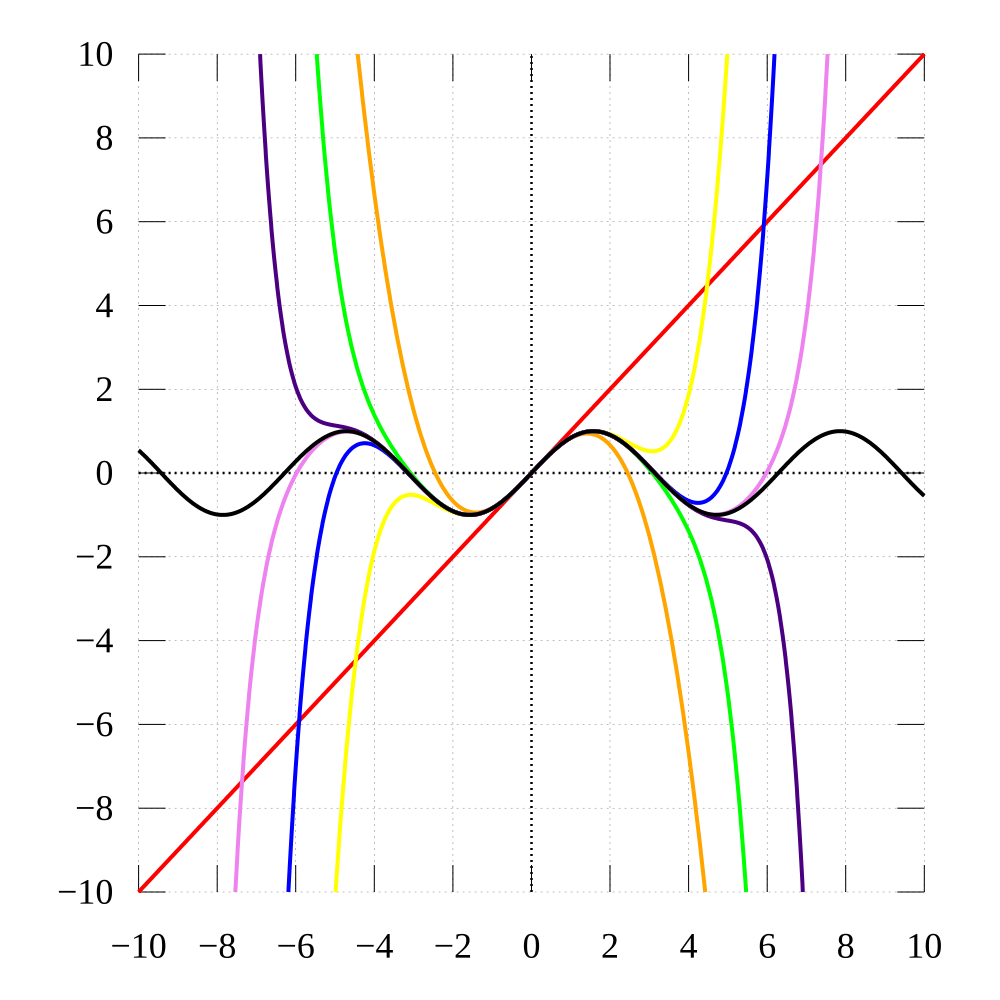
\includegraphics[width=0.25\textwidth]{Images/taylor.png}
  \caption{Taylor approximation to of orders 1 to 7 of the function $\sin(x)$ (Source: Wikipedia)}
  \Description{}
\end{figure}

Let's now suppose that our function is two-dimensional $f(\boldsymbol x)$, and
that it is defined on a discrete grid of $(I\times J)$ points $\boldsymbol
  x_{i,j} = \qty(x_i, \ y_j)^T = \qty(i \, \Delta x, \ j \, \Delta y)^T$, where
$i = 1, \dots, I$ and $j = 1, \dots, J$. This is called our
\textit{computational mesh}, and is the domain on which our functions of
interest will be defined.

\begin{figure}[H]
  \centering
  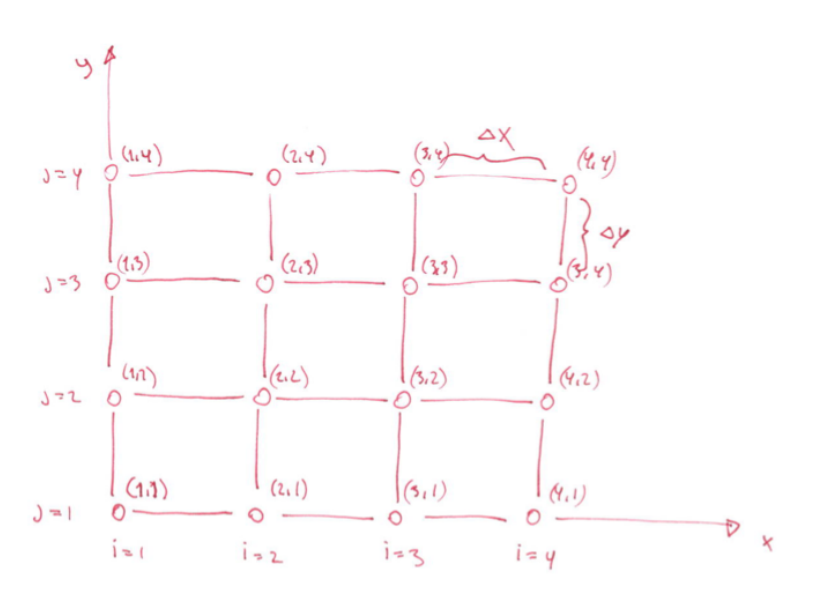
\includegraphics[width=0.3\textwidth]{Images/computational mesh.png}
  \caption{The computational mesh}
  \Description{}
\end{figure}

The value of the function in a point on the grid is denoted by $f(\boldsymbol
  x_{i,j}) = f_{i,j}$. Given that we know the value of the function in the points
$\boldsymbol x_{i,j}$ and $\boldsymbol x_{i+1,j}$, we can approximate it's
partial derivatives in $\boldsymbol x_{i,j}$ by using Equation
(\ref{eq:taylordiff})
%
\begin{subequations}
  \begin{equation}
    \pdv{f_{i,j}}{x} \approx \frac{f_{i+1,j} - f_{i,j}}{\Delta x},
  \end{equation}
  \begin{equation}
    \pdv{f_{i,j}}{x} \approx \frac{f_{i+1,j} - f_{i,j}}{\Delta x},
  \end{equation}
  \label{eq:FDA}
\end{subequations}
%
This is called the \textit{forward difference approximation} (FDA) as it looks
\textit{forwards} in the direction of the derivative to approximate. The
\textit{backward difference approximation} (BDA) is derived in a similar way,
but looks \textit{backwards} in the direction of the derivative to approximate
and is defined as such
%
\begin{subequations}
  \begin{equation}
    \pdv{f_{i,j}}{x}  \approx \frac{f_{i,j} - f_{i-1,j}}{\Delta x},
  \end{equation}
  \begin{equation}
    \pdv{f_{i,j}}{y} \approx \frac{f_{i,j} - f_{i,j-1}}{\Delta y}.
  \end{equation}
  \label{eq:BDA}
\end{subequations}
%
If we take Equations (\ref{eq:FDA}) and (\ref{eq:BDA}) and add them together,
we get
%
\begin{subequations}
  \begin{equation}
    \pdv{f_{i,j}}{x} \approx \frac{f_{i+1,j} - f_{i-1,j}}{2\Delta x},
  \end{equation}
  \begin{equation}
    \pdv{f_{i,j}}{y} \approx \frac{f_{i+1,j} - f_{i-1,j}}{2\Delta y}.
  \end{equation}
\end{subequations}
%
This is called the \textit{central difference approximation} (CDA). One of the
benefits of the CDA is that it doesn't favor any directions when approximating
the derivative, and thus it is more reliable than the FDA and BDA.

Using the CDA we may approximate the second derivative of $f_{i,j}$ as
%
\begin{align}
  \pdv[2]{f_{i,j}}{x}  \approx \frac{\pdv{f_{i+\frac12, j}}{x} - \pdv{f_{i-\frac12, j}}{x}}{\Delta x} & \approx \frac{f_{i+1, j} - f_{i, j} - \qty(f_{i,j} - f_{i - 1, j})}{\Delta x^2},
\end{align}
%
where we've used discrete steps of size $\Delta x/2$ and $\Delta y/2$. This
would imply a finer grid, but as we shall see this effect goes out in the final
expression. Our expression now yields the approximation of the second order
derivatives of our function $f$ in the point $\boldsymbol x_{i,j}$
%
\begin{subequations}
  \begin{equation}
    \pdv[2]{f_{i,j}}{x} \approx \frac{f_{i+1, j} - 2f_{i,j} + f_{i-1,j}}{\Delta x^2},
  \end{equation}
  \begin{equation}
    \pdv[2]{f_{i,j}}{y} \approx \frac{f_{i, j+1} - 2f_{i,j} + f_{i,j-1}}{\Delta y^2}.
  \end{equation}
\end{subequations}
%
We see that any dependence on the finer grid of half steps has disappeared.

\section{Numerical solution}
\subsection{Formulation of the linear system}
Using the first order and second order derivative approximations derived above,
we can write the finite difference approximation to the governing equation
(\ref{eq:governing}) as
%
\begin{equation}
  \frac{u_{i+1,j} - 2u_{i,j} + u_{i-1,j}}{\Delta x^2} + \frac{u_{i,j+1} - 2u_{i,j} + u_{i,j-1}}{\Delta y^2} - k^2 u_{i,j} = f_{i,j}.
  \label{eq:app_governing}
\end{equation}
%
Rearrainging this we obtain the equation
%
\begin{multline}
  \underbrace{ \frac{1}{\Delta y^2}}_{ c_{i,j-1} } u_{i,j-1} + \underbrace{ \frac{1}{\Delta x^2} }_{ c_{i-1,j} } u_{i-1,j} + \underbrace{ \frac{1}{\Delta x^2} }_{ c_{i+1,j} } u_{i+1,j} + \underbrace{ \frac{1}{\Delta y^2} }_{ c_{i,j+1} } u_{i,j+1}\\
  + \underbrace{\left(- k^2 - \frac{2}{\Delta x^2} -\frac{2}{\Delta y^2}\right) }_{ c_{i,j} } u_{i,j} = f_{i,j}.
  \label{eq:lin_sys}
\end{multline}
%
This equation is a linear combination the values of $u$ at the neighbouring
points and the point itself, with the coefficients $c_{i,j-1}$, $c_{i-1,j}$,
$c_{i+1,j}$, $c_{i,j+1}$, and $c_{i,j}$ and holds true for all points on our
computational mesh except the boundary poitns which we will deal with shortly.
The collection of points $u_{i-1,j}$, $u_{i+1,j}$, $u_{i,j-1}$, $u_{i,j+1}$,
and $u_{i,j}$ is called the stencil, and can be thought of as a geometrical
``filter'' moving around on top of our grid telling us which points affect the
solution at the point in the center.

\begin{figure}[H]
  \centering
  \includegraphics[width=0.3\textwidth]{Images/stencil.png}
  \caption{The stencil of the point $u_{i,j}$}
  \Description{}
\end{figure}

Equivalent to Equation (\ref{eq:lin_sys}) is the expression
%
\begin{multline}
  u_{i,j} = g(u_{i,j}) = \frac{1}{c_{i,j}} \Big[f_{i,j} - c_{i-1,j} u_{i-1,j} - c_{i+1,j} u_{i+1,j}\\
    - c_{i,j-1} u_{i,j-1} - c_{i,j+1} u_{i,j+1}\Big],
\end{multline}
%
which is called an \textit{update formula} and defines our \textit{update
  scheme} as such
%
\begin{equation}
  u_{i,j}^{k+1} = g(u_{i,j}^k)
\end{equation}
%
where $g$ is an affine function and $k$ is the iteration number. Our update
scheme describes a \textit{fixed point problem}, which can be reformulated as a
matrix equation
%
\begin{equation}
  \boldsymbol A \boldsymbol u = \boldsymbol f, \label{eq:matrix_eq}
\end{equation}
%
where $\boldsymbol A$ is an \( (I \cdot J \times I \cdot J) \), where each row
holds all the coefficients $c_{i,j}$ corresponding to a given point $u_{i,j}$
and $\boldsymbol u$ and $\boldsymbol f$ are \( (1\times I \cdot J) \) vectors
that holds the values of $u$ and $f$ at all points on the grid. This is called
the matrix assembly and in our case it looks like Figure~\ref{fig:A_matrix}.

\begin{figure}[H]
  \centering
  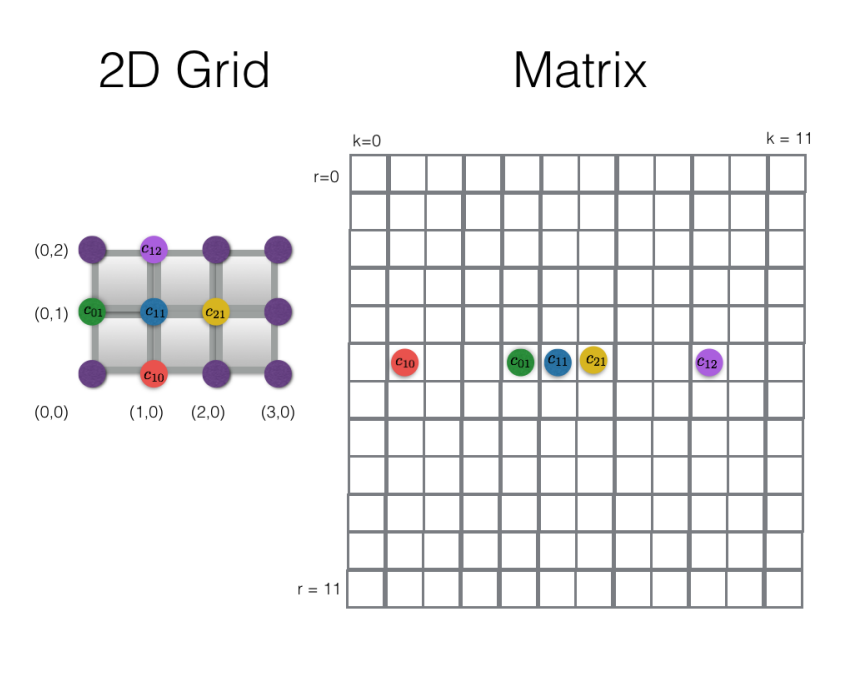
\includegraphics[width=0.4\textwidth]{Images/grid_to_matrix.png}
  \caption{The concatenation of multiple instances of the computational grid into a matrix.}
  \Description{}
\end{figure}

\begin{figure}[H]
  \centering
  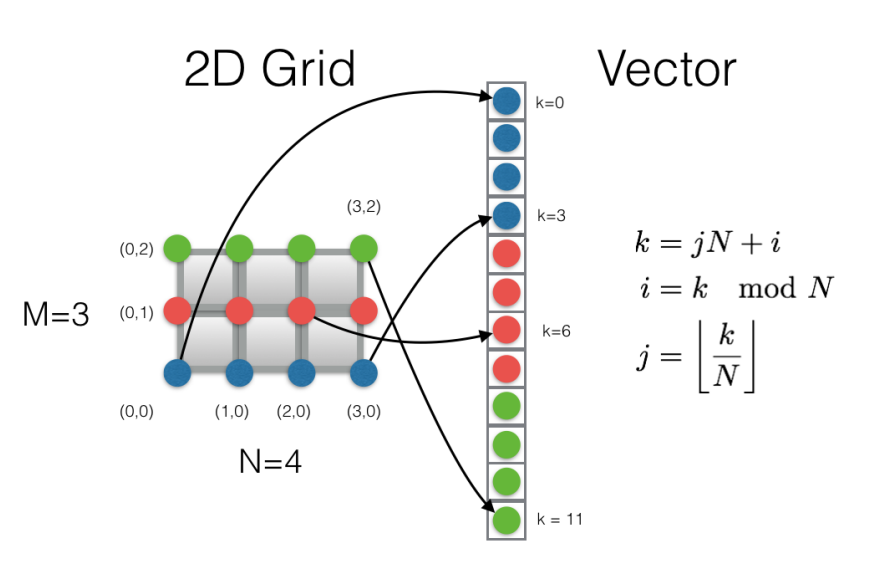
\includegraphics[width=0.4\textwidth]{Images/grid_to_vector.png}
  \caption{The transformation of the computational grid into a vector.}
  \Description{}
\end{figure}

\subsection{Boundary conditions}
While filling the $\boldsymbol A$ matrix in the matrix assembly, we need to pay
special attention to the boundaries, as our stencil is not well defined here.
At least one of the ``arms'' of the stecil will reach outside the domain, and
thus have an undefined value.

\begin{figure}[H]
  \centering
  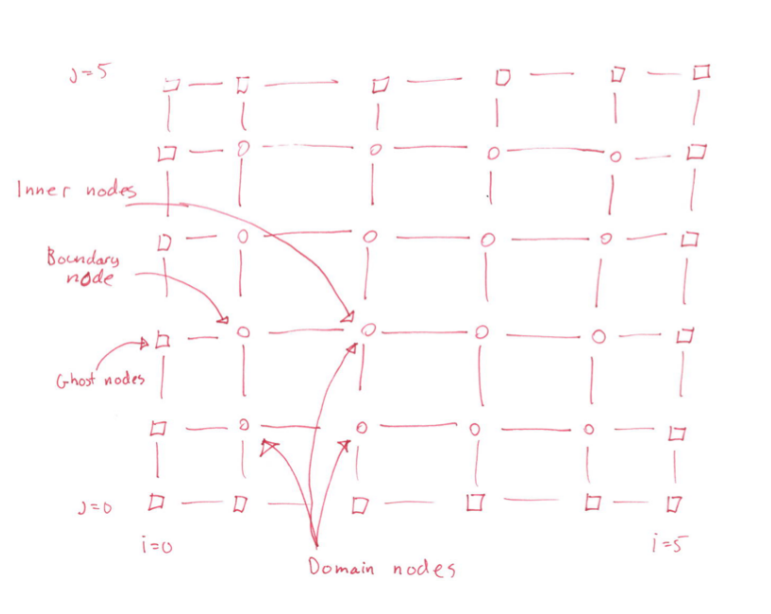
\includegraphics[width=0.3\textwidth]{Images/ghost_nodes.png}
  \caption{Computational mesh with a layer of ghost nodes on the outside.}
  \Description{}
\end{figure}

To deal with this, we will introduce a layer of \textit{ghost nodes} outside
our domain, the values of which we will set according to a set of von Neumann
boundary conditions defined as
%
\begin{equation}
  \pdv{u}{n} = 0,
\end{equation}
%
where $n$ is the normal to the boundary. This means that the derivative of $u$
across the boundary is zero. In the finite difference approximation, this
equates to the value of the ghost nodes being equal to the value of the
boundary nodes, since
%
\begin{align}
           &  & \pdv{u}{n}       & \approx \frac{u_\mathrm{boundary} - u_\mathrm{ghost}}{\Delta x} = 0 \hspace{30pt} \\
  \implies &  & u_\mathrm{ghost} & = u_\mathrm{boundary}.
\end{align}
%
Using the FDA or BDA depending on which boundary we are dealing with, we can
derive for each of the four boundaries of our domain that
%
\begin{align}
  \text{Left boundary:}  &  & u_{0,j} = u_{1,j}, \notag     \\
  \text{right boundary:} &  & u_{I-1, j} = u_{I, j}, \notag \\
  \text{lower boundary:} &  & u_{i,0} = u_{i,1}, \notag     \\
  \text{upper boundary:} &  & u_{i, J-1} = u_{i, J}.
\end{align}
%
Now we have a complete $\boldsymbol A$-matrix, and we can solve the linear
system.

\begin{figure}[H]
  \centering
  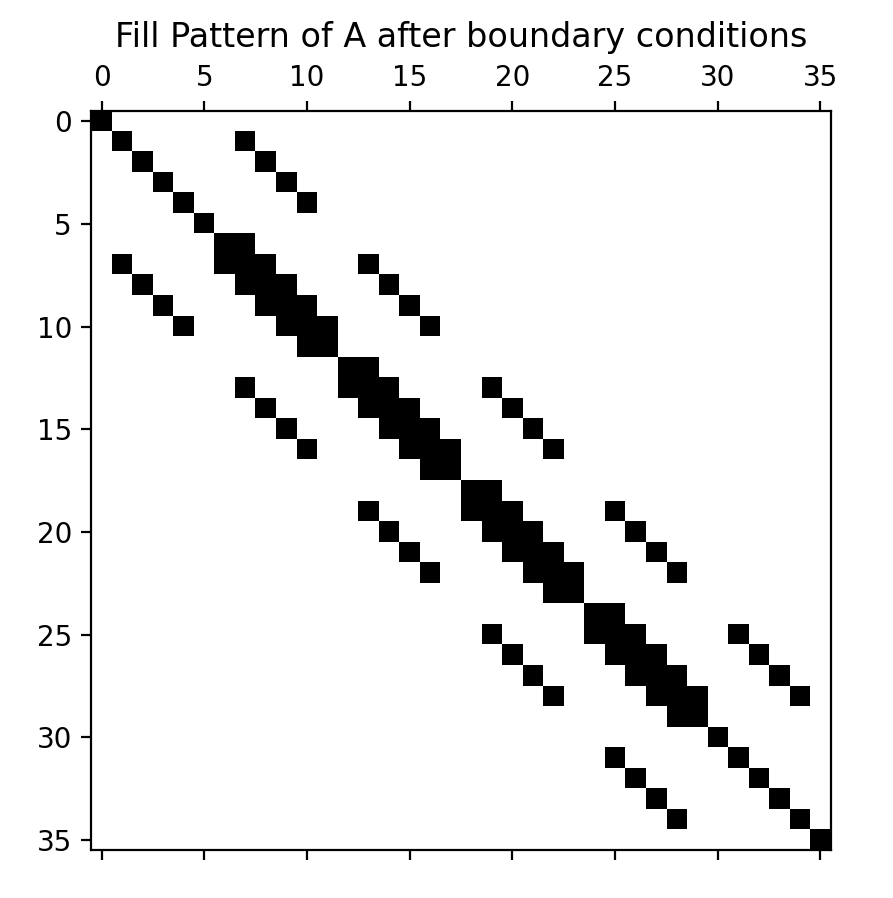
\includegraphics[width=0.2\textwidth]{Images/A_matrix.png}
  \caption{Example of final $\boldsymbol A$-matrix for a domain of size $(4 \times 4)$.\label{fig:A_matrix}}
\end{figure}

\section{Verification}
To make sure that our interpretation of the mathematical model
(\ref{eq:governing}) as a matrix equation (\ref{eq:matrix_eq}) is correct,
we'll do two experiments trying to verify our implementation.

\subsection{Experiment 1: Limiting case}
One simple way to verify that our matrix equation represents our mathematical
model, is to test the limiting case where $|- k^2 u| \gg |\nabla^2 u|$. Since
$\nabla^2 \sim 1/dx^2$, this means that we want to set $k \gg 1/dx$.

Here Equation (\ref{eq:governing}) becomes
\begin{equation}
  -k^2 u = f,
\end{equation}
which means that the solution $u$ should be proportional to our input $f$.
Let $k = 100$ and
%
\begin{subequations}
  \begin{align}
    f_1(x,y) & = x + y                          \\
    f_2(x,y) & = x^2 - y^2                      \\
    f_3(x,y) & = \sin(2 \pi x) + \cos(2 \pi y).
  \end{align}
\end{subequations}
%
In the first case we expect our solution to be a slanted plane, in the second
it should be a saddle, and in the third it should be a sinusoidal wave in both
dimensions.

With a grid of dimension $(100 \times 100)$ mapping onto $x,y \in [-1, 1]$, we
have $1/dx = 1/dy = 50$, and thus $k \gg 1/dx$ holds for $k = 100.000$. We will
use this value for all three cases.

\begin{figure}[H]
  \centering
  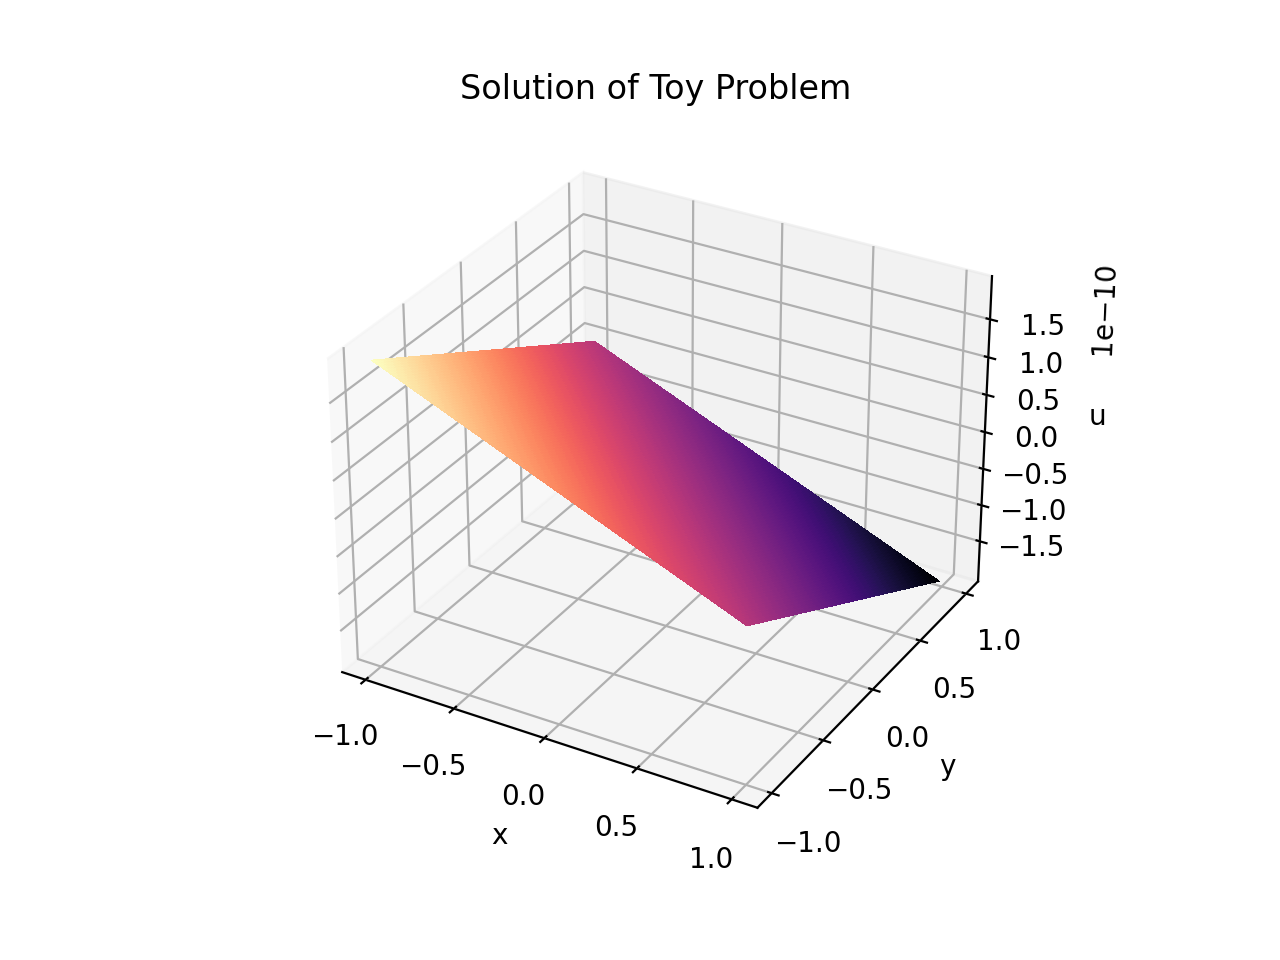
\includegraphics[width=0.3\textwidth]{Images/plane_sol.png}
  \caption{Solution to the week 1 problem with $k=10000$, $f(x,y) = x + y$, and computational mesh with dimensions $(100 \times 100) \to [-1, 1]$.\label{fig:plane}}
\end{figure}
\begin{figure}[H]
  \centering
  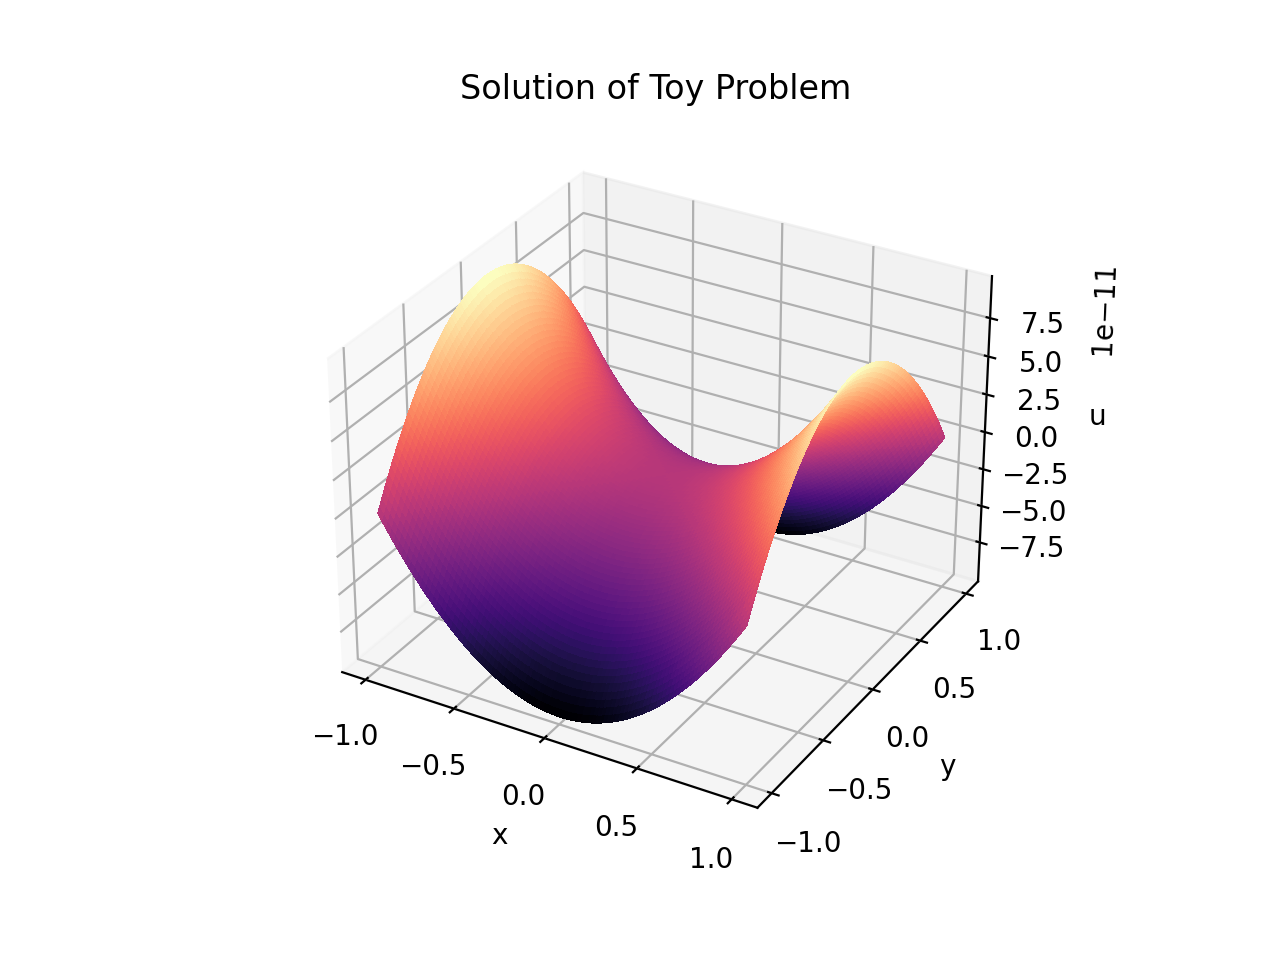
\includegraphics[width=0.3\textwidth]{Images/quad_sol.png}
  \caption{Solution to the week 1 problem with $k=10000$, $f(x,y) = x^2 - y^2$, and computational mesh with dimensions $(100 \times 100) \to [-1, 1]$.\label{fig:saddle}}
\end{figure}
\begin{figure}[H]
  \centering
  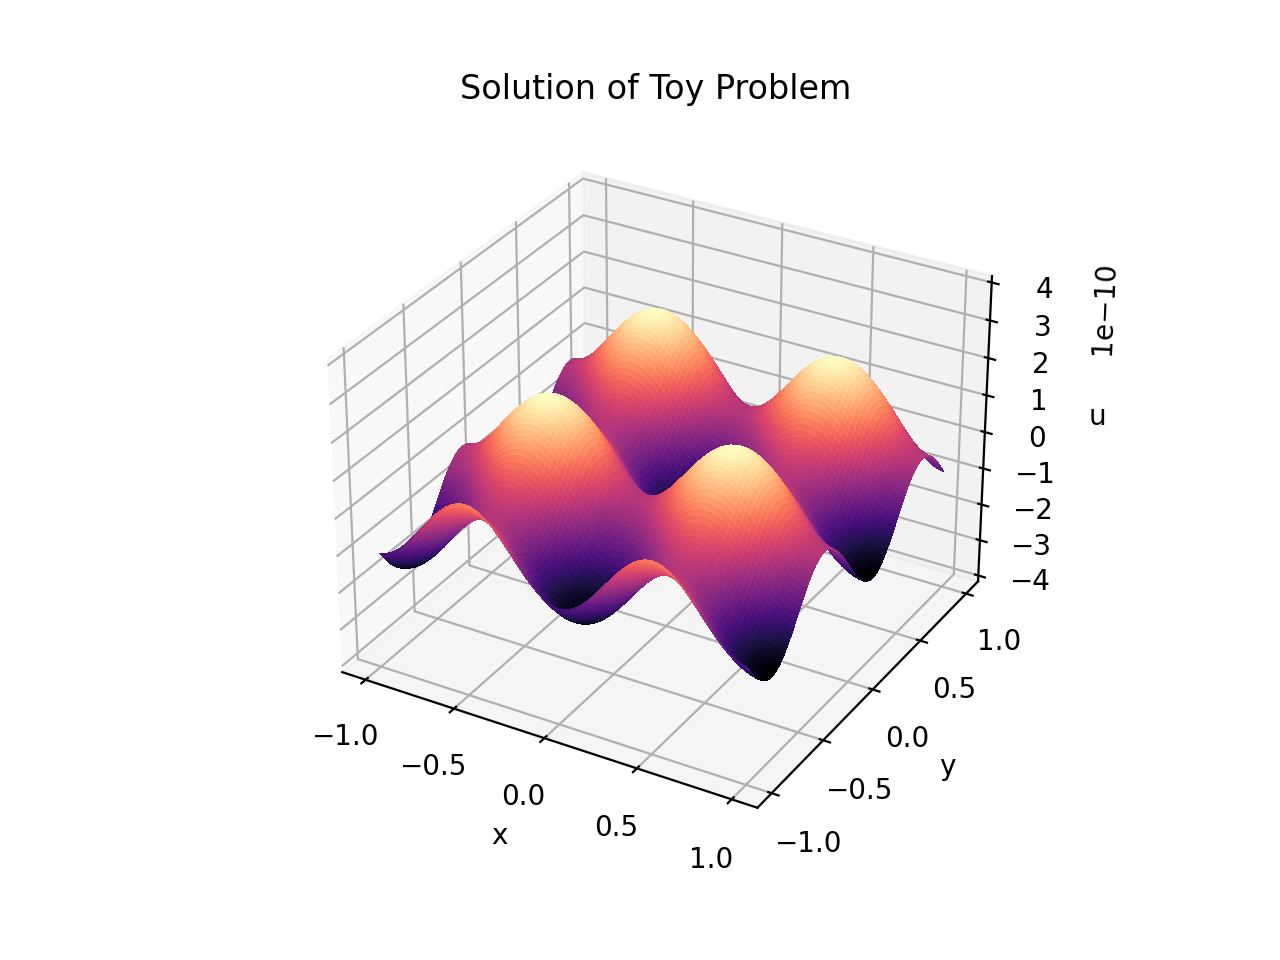
\includegraphics[width=0.3\textwidth]{Images/wave_sol.png}
  \caption{Solution to the week 1 problem with $k=10000$, $f(x,y) = \sin(2\pi x) + \cos(2\pi y)$, and computational mesh with dimensions$(100 \times 100) \to [-1, 1]$.\label{fig:wave}}
\end{figure}

In Figures~\ref{fig:plane},~\ref{fig:saddle}, and~\ref{fig:wave} we see that
the solutions $u$ are endeed proportional to the known $f$. This agrees wit the
mathematical model, and is therefore a verification of our implementation.

\subsection{Experiment 2:}
As another experiment let's examine the contribution of the term with the
laplacian. We will use the value $k = 1$ and do the simulation for the linear
function $f_1$ and for a step function $f_2$, defined as such
%
\begin{align}
  f_1(x,y) & = x + y                                           \\
  f_2(x,y) & = \begin{cases}
                 1 & \text{if } x \in [-1, 0] \land y \in [0, 1] \\
                 0 & \text{otherwise}.
               \end{cases}
\end{align}
%
\begin{figure}[H]
  \centering
  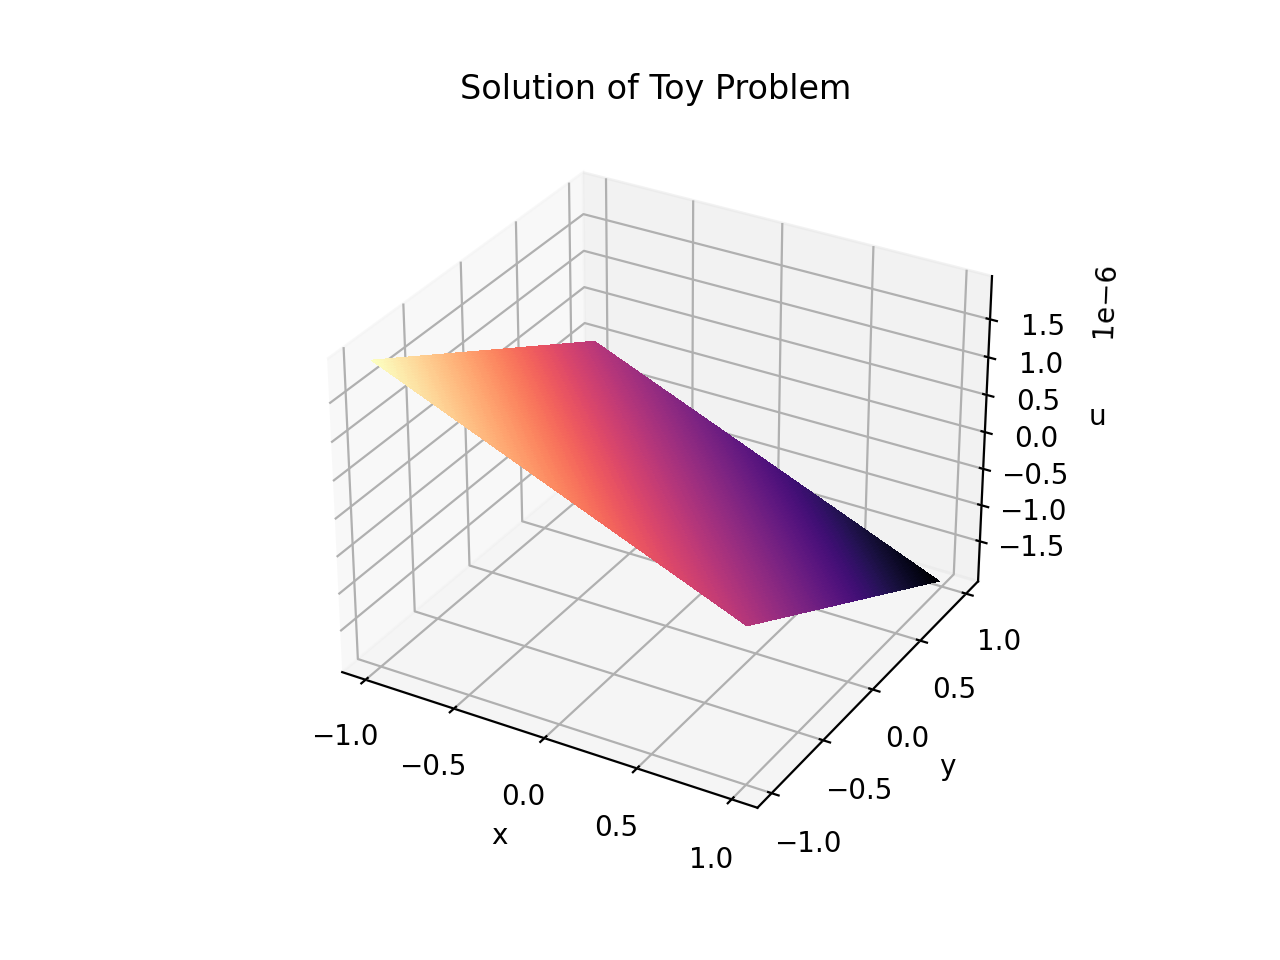
\includegraphics[width=0.3\textwidth]{Images/exp1_plane_k.png}
  \caption{Plot of $-k^2 u = f$ with $k=1$ and $f_1 = x+y$.~\label{fig:exp1_plane_k}}
\end{figure}
\begin{figure}[H]
  \centering
  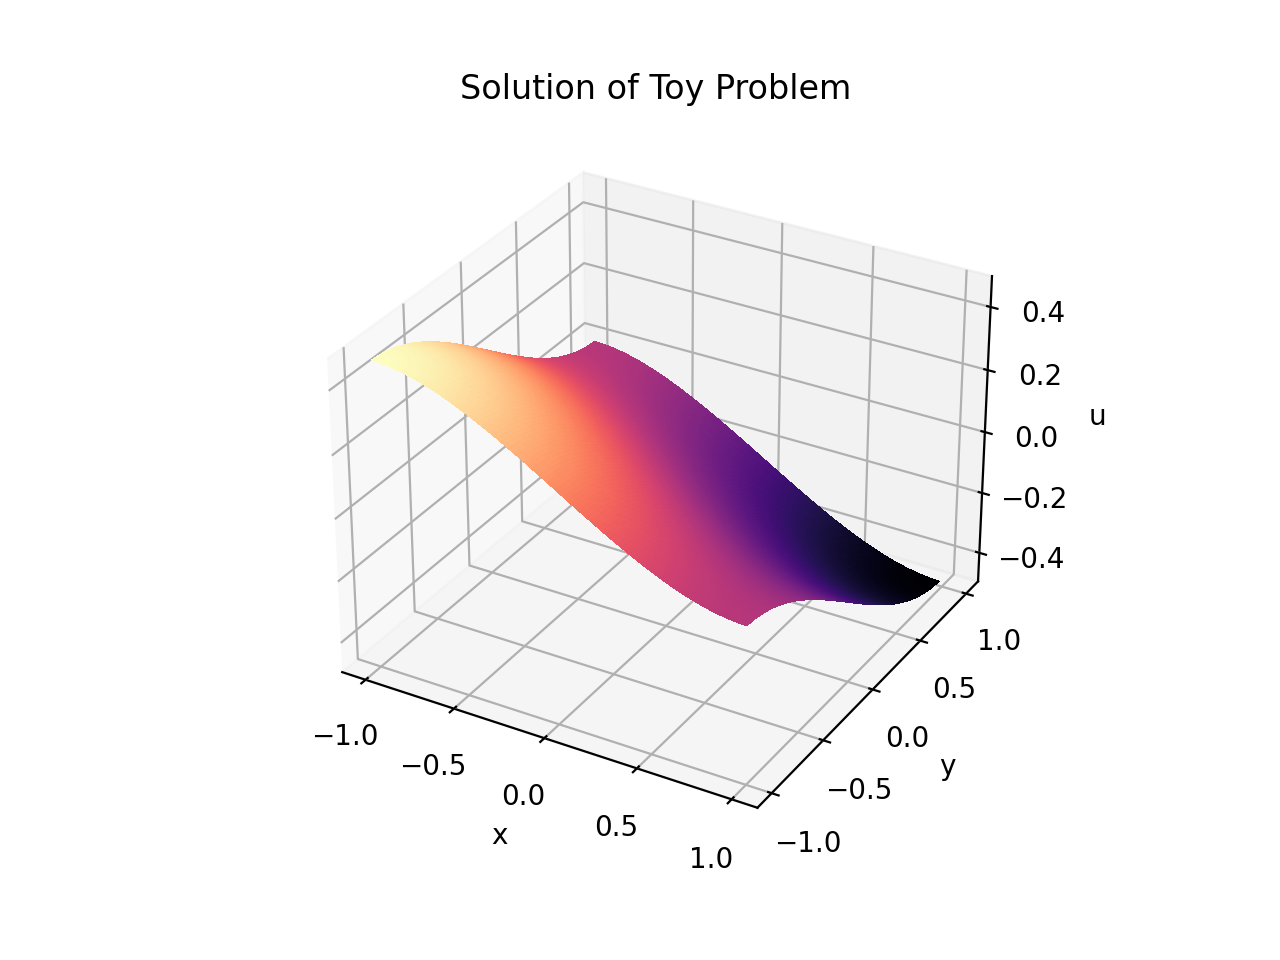
\includegraphics[width=0.3\textwidth]{Images/exp1_plane_full.png}
  \caption{Plot of full solution with $k=1$ and $f_1 = x+y$.~\label{fig:exp1_plane_full}}
\end{figure}
\begin{figure}[H]
  \centering
  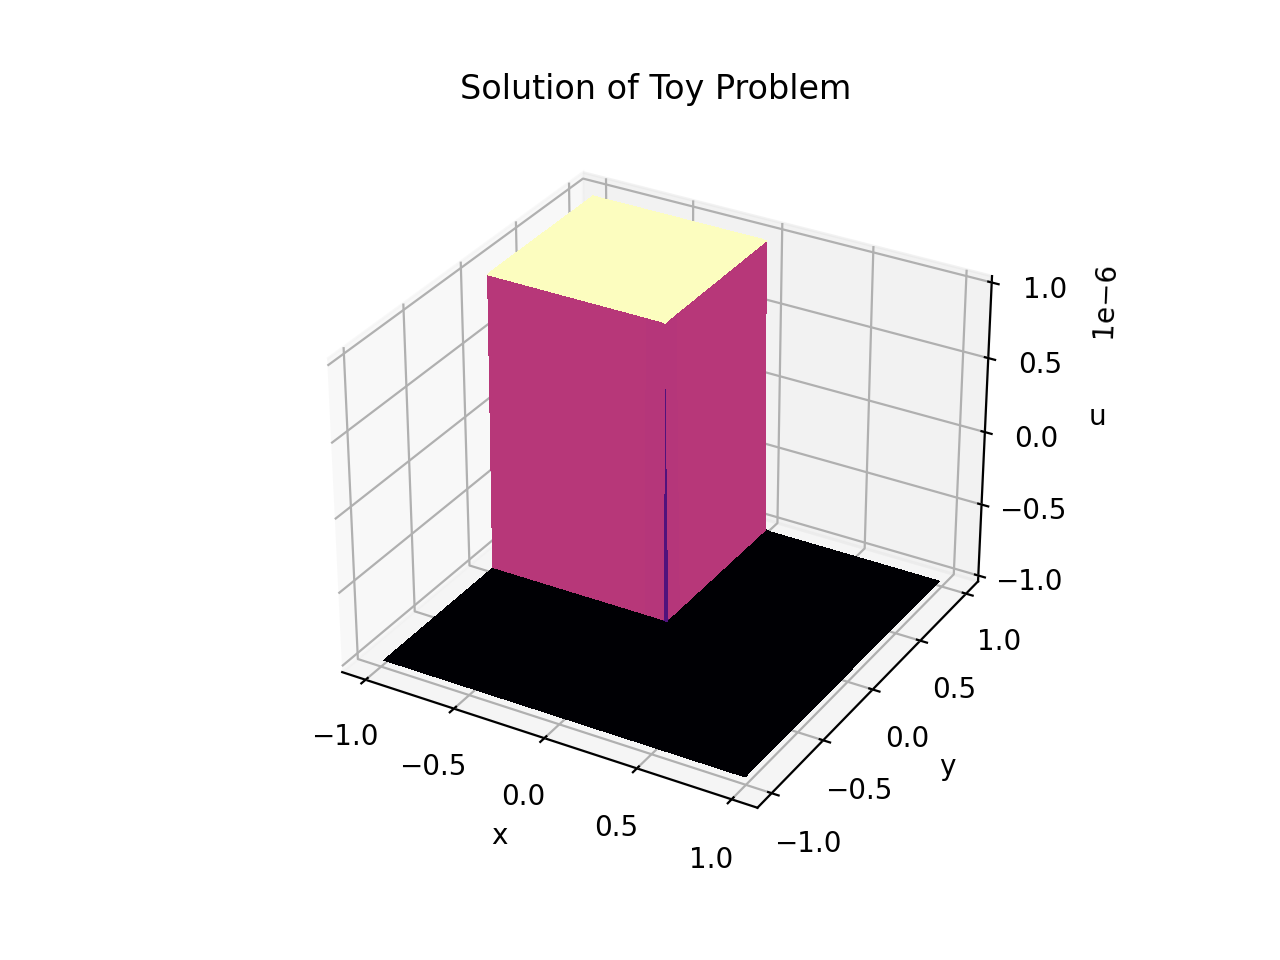
\includegraphics[width=0.3\textwidth]{Images/exp1_step_k.png}
  \caption{Plot of $-k^2 u = f$ with $k=1$ and the step function $f_2$.~\label{fig:exp1_step_k}}
\end{figure}
\begin{figure}[H]
  \centering
  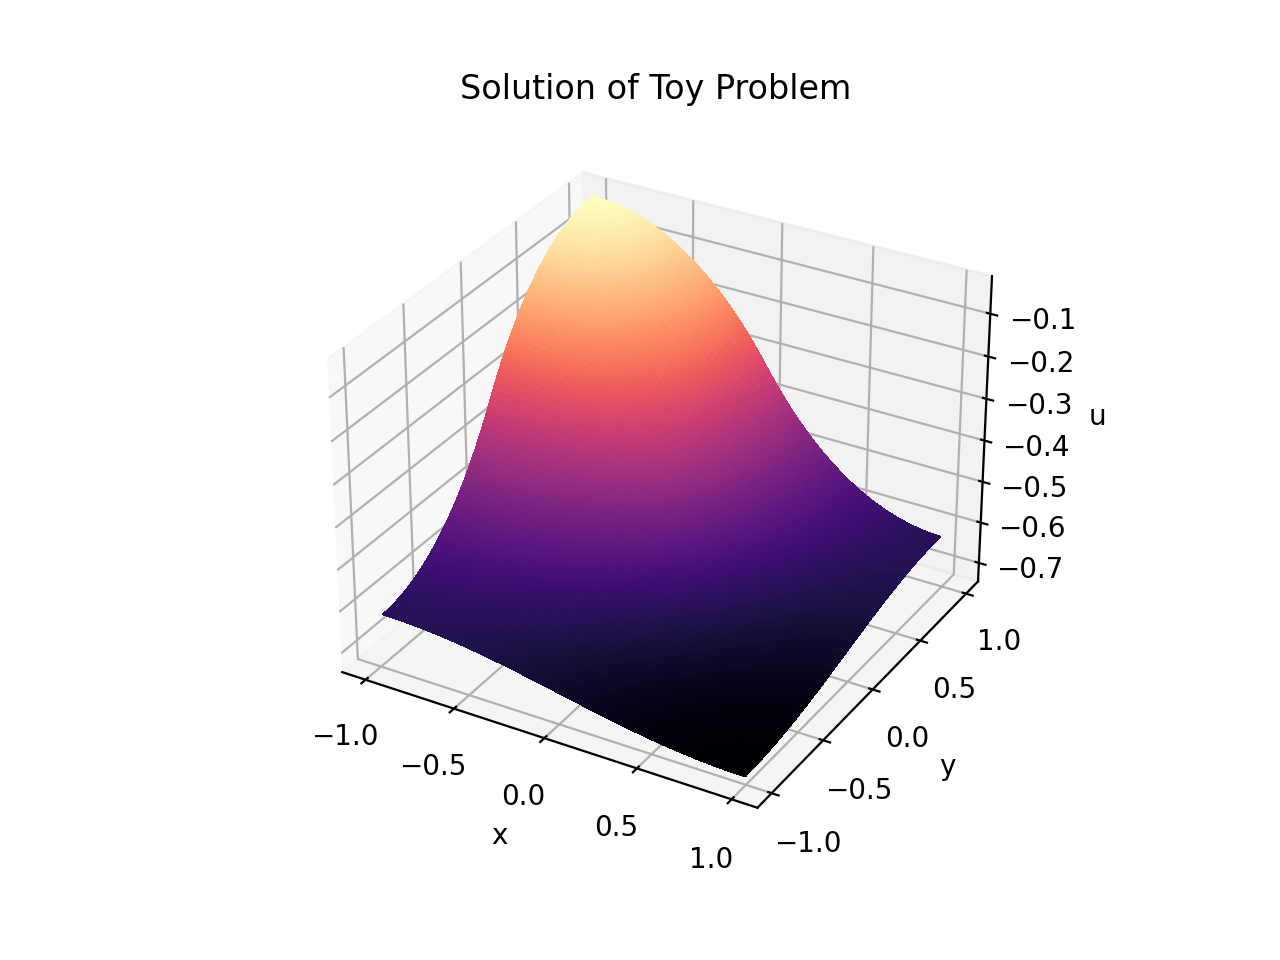
\includegraphics[width=0.3\textwidth]{Images/exp1_step_full.png}
  \caption{Plot of full solution with $k=1$ and the step function $f_2$.~\label{fig:exp1_step_full}}
\end{figure}

We see that in the case where $f$ has a big continuity, the full solution
differs alot from only the $-k^2 u = f$ plot. This is expected as the laplacian
term will be of greater magnitude when the discontinuity is great. This agrees
wit the mathematical model, and is therefore another verification of our
implementation.

\newpage
\section*{Week 2: Introduction}

In this section of the report we will seek to find a numerical solution to the
equations
\begin{align}
   & \text{Advective flow:}      & \frac{D \phi}{Dt} & = (\boldsymbol u \cdot \nabla) \phi + \frac{\partial \phi}{\partial t} = 0,
  \label{eq:advection}                                                                                                                                                              \\
   & \text{Mean curvature flow:} & \pdv{\phi}{t}     & = -2 \boldsymbol \nabla \cdot \frac{\boldsymbol \nabla \phi}{\left\lVert \boldsymbol \nabla \phi \right\rVert } = - 2 \kappa
  \label{eq:mean_curvature}
\end{align}

\section{Advection}
\subsection{Semi-Lagrangian time integration}
Advection is the process of transporting a quantity, such as a fluid variable
or a scalar field, along the flow of a velocity field. Therefore it can be
benificial to solve this problem from the perspective of the fluid particles.
This is the idea behind the \textit{semi-Lagrangian time integration}.

Given the velocity field $\boldsymbol u(\boldsymbol x, t)$, we can trace where
the particle, that is currently in the grid point of our model, was at the
previous time step with a simple implicit Euler step:
%
\begin{align}
  \boldsymbol x^{t-\Delta t} = \boldsymbol x^t - \boldsymbol u(\boldsymbol x^t, t) \, \Delta t.
\end{align}
%
Then we infer the value of the quantity we are interested in (in our case
$\phi$), at the point of the particle $\boldsymbol x^{t -\Delta t}$, by
interpolating the values of $\phi$ at the nearest neighbouring grid points. We
then update the value of the quantity at the grid point $\boldsymbol x^{t}$ to
be the interpolated value with this expression
%
\begin{align}
  \phi^{t} = \phi^{t-\Delta t} + k \, \Delta t = \phi^{t-\Delta t},
\end{align}
%
since in our case $k = (\boldsymbol u \cdot \nabla) \phi + \frac{\partial
    \phi}{\partial t} = 0$.

\section{Verification}
\subsection{Experiment 1: Grid and time step sizes}

When using the semi-Lagrangian integration scheme we have to be aware of any
numerical diffusion effects caused by the interpolation and discrete time
steps. We will now examine this effect by varying the time step $\Delta t$ and
the grid size $\Delta x$ and keeping track of the numerical error. We know what
the error should be, since we assume $\phi$ to be conserved, which means that
the volume should stay the same over the integration period. We can then
calculate the error of a given simulation as the difference in volume before
and after simulating.

We will simulate for the values $\Delta t = [0.05, 0.01, 0.02]$ and $N = [32,
  64, 128]$.

\begin{figure}[H]
  \centering
  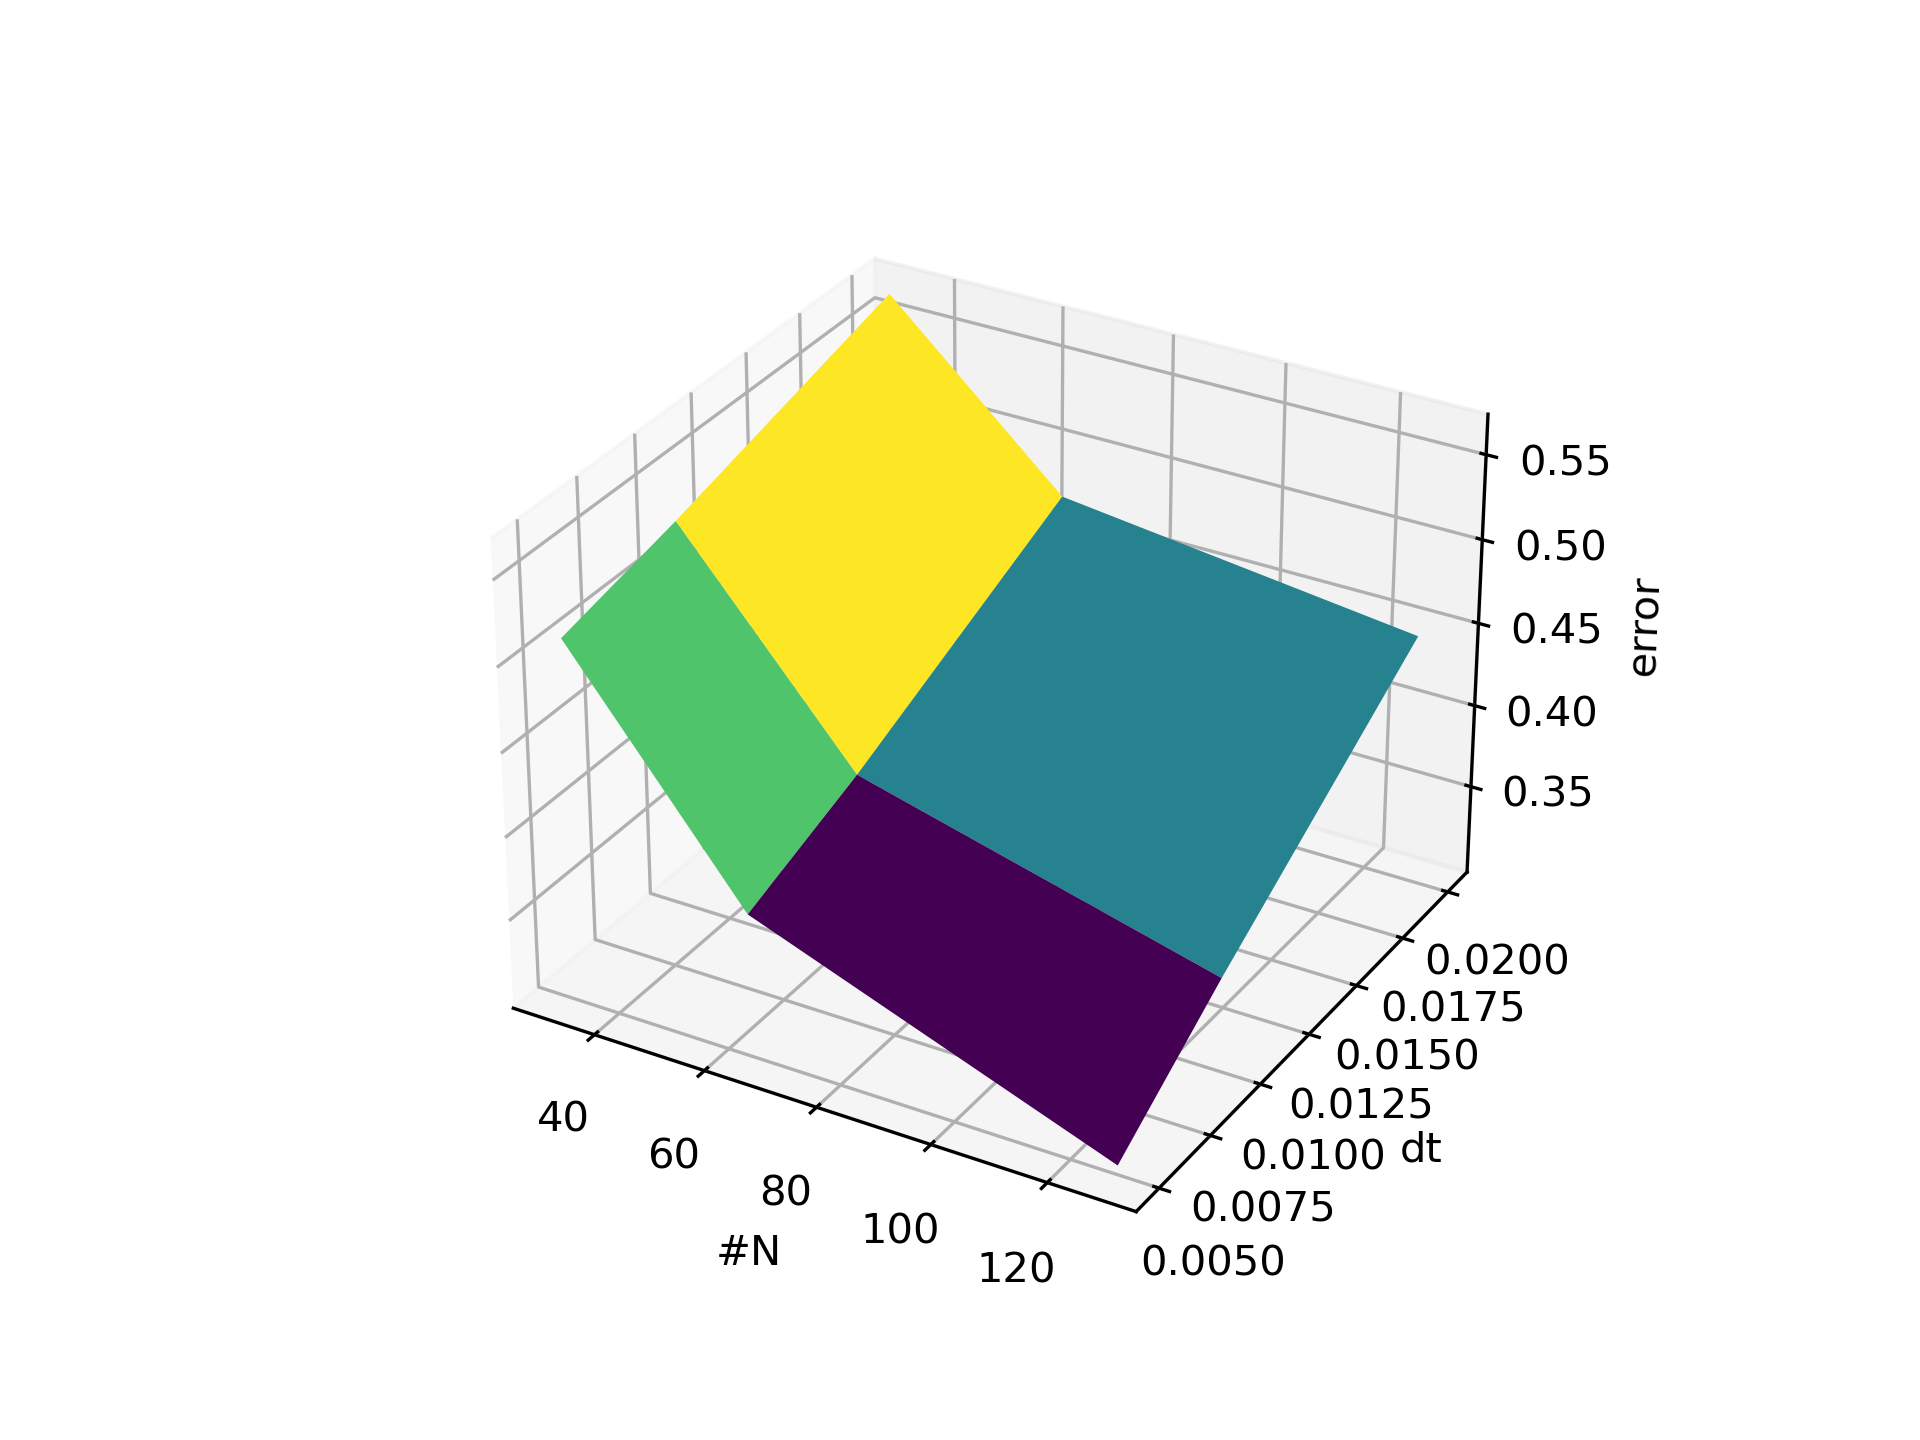
\includegraphics[width=0.3\textwidth]{Images/advection/exp1_errors.png}
  \caption{A plot of the errors produced by the advection simulation for different grid divisions $N = [32, 64, 128]$ and time step sizes $\Delta t = [0.05, 0.01, 0.02]$. The minimum error was 0.302, and the maximum error was 0.568}
  \label{fig:adv_exp1_errors}
\end{figure}

It is clear from Figure~\ref{fig:adv_exp1_errors} that the error decreases as
the time step gets smaller and the grid gets finer, i.e. $N \to \infty$ and $dt
  \to 0$. This is expected, as the interpolation error decreases as the grid gets
finer, and the numerical diffusion decreases as the time step gets smaller. We
also see that increasing the grid size has a larger effect on the error than
decreasing the time step size.

The velocity field we used to advect $\phi$ with, is given by $\boldsymbol u =
  \qty(y, -x)$, which is a rotational field. This means that ideally $\phi$
should only rotate around the origin, and it's volume shouldn't change. We
simulated a full rotation of the field. In reality, for the grid sizes and time
steps we simulated with, we expect a significant error, and we expect it to be
larger for the larger grid sizes due to numerical diffusion.

\begin{figure}[H]
  \centering
  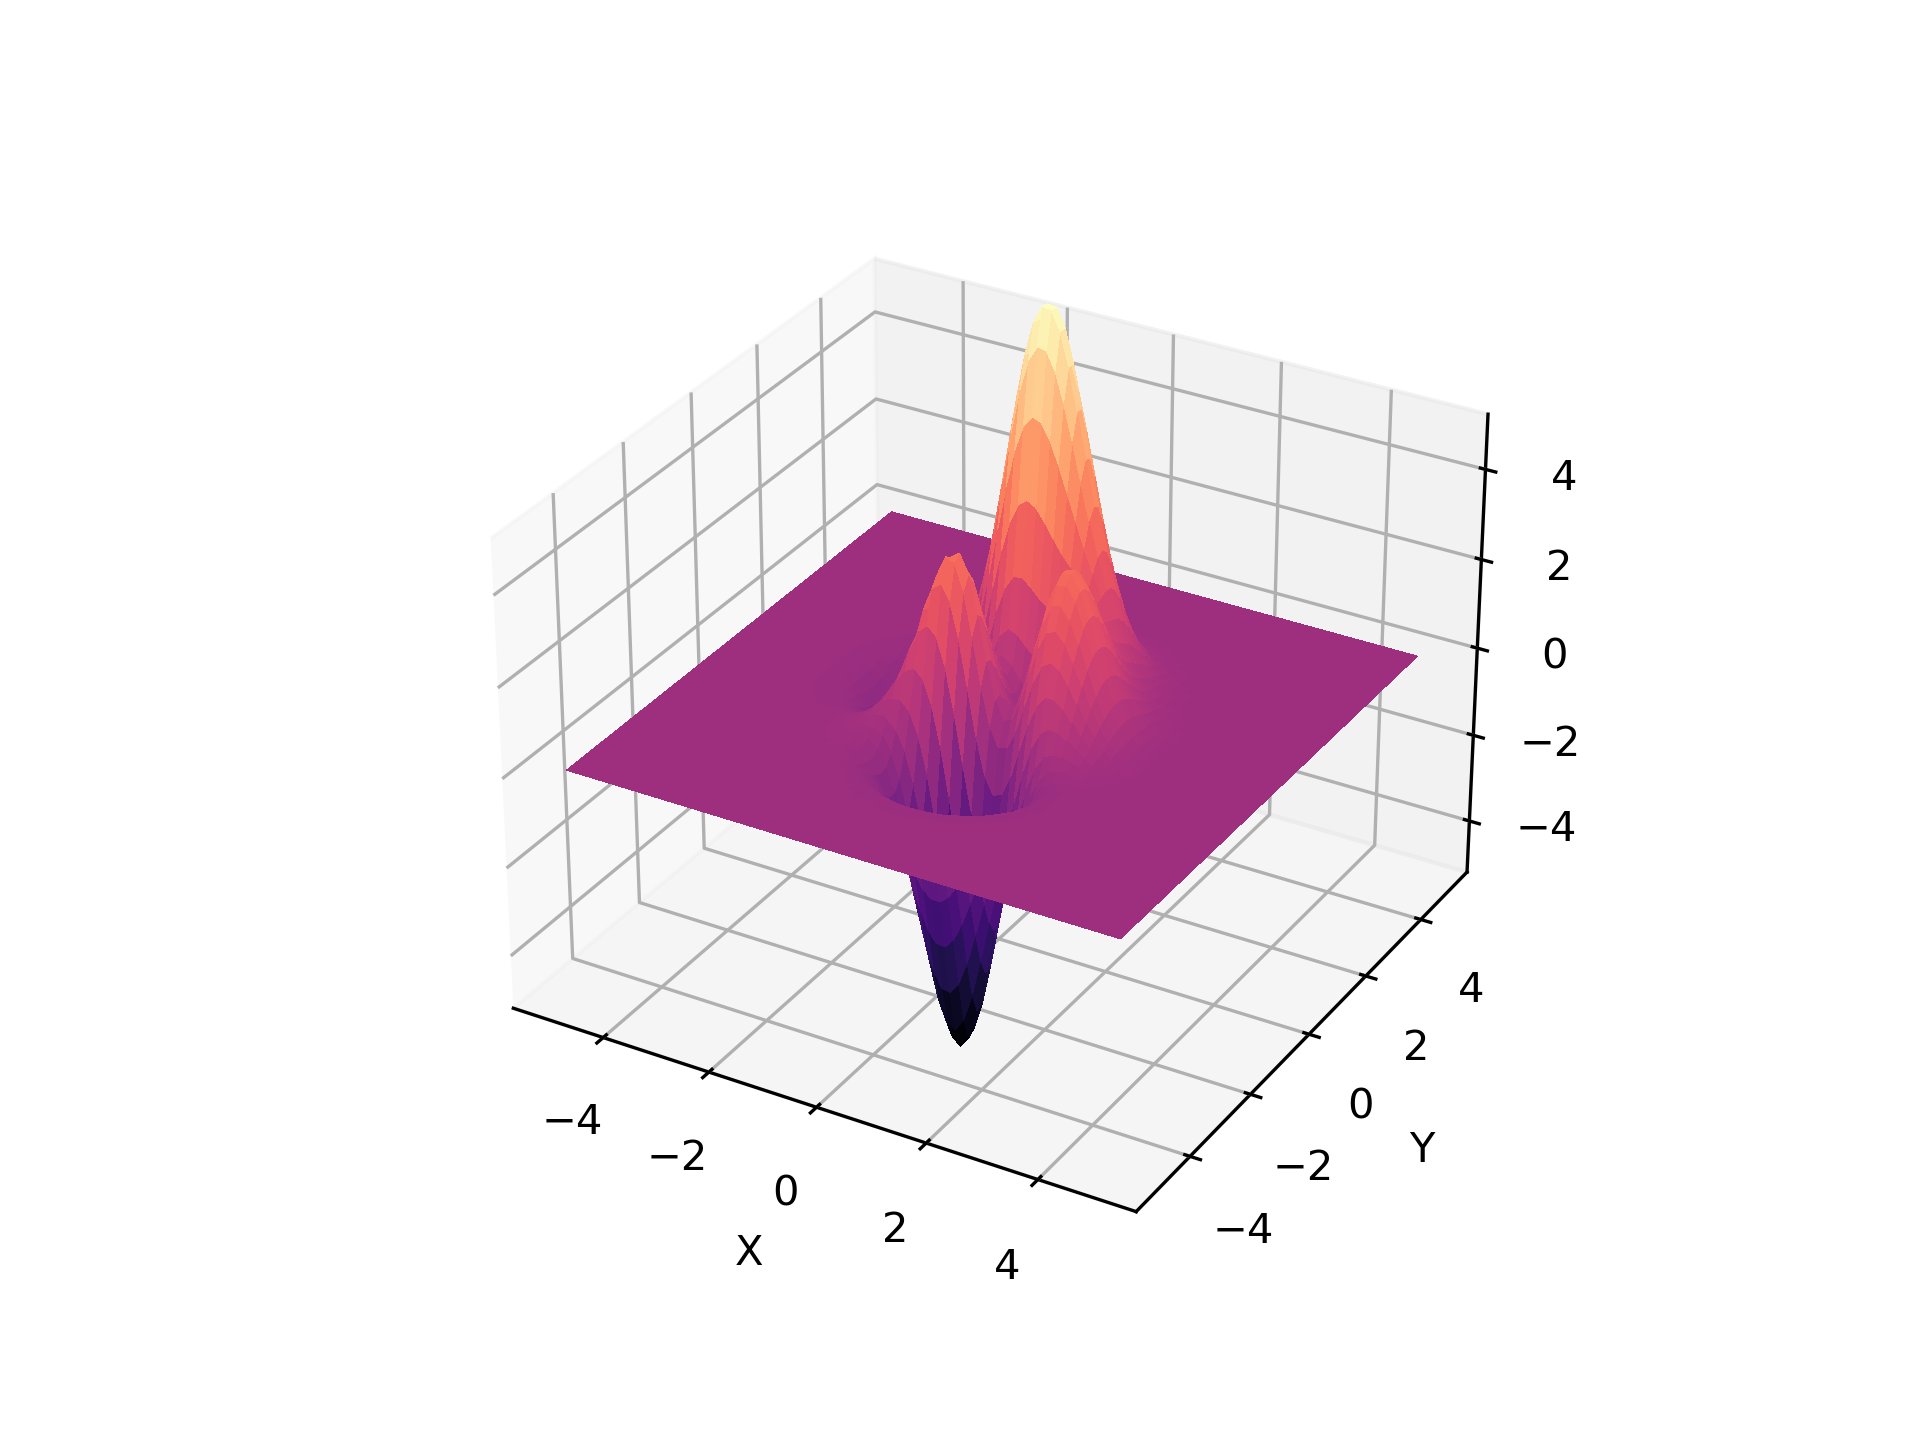
\includegraphics[width=0.3\textwidth]{Images/advection/exp1_I_64_start.png}
  \caption{Initial conditions for the advection problem with $N=64$, $dt = 0.05$.\label{fig:adv_exp1_start}}
\end{figure}
\begin{figure}[H]
  \centering
  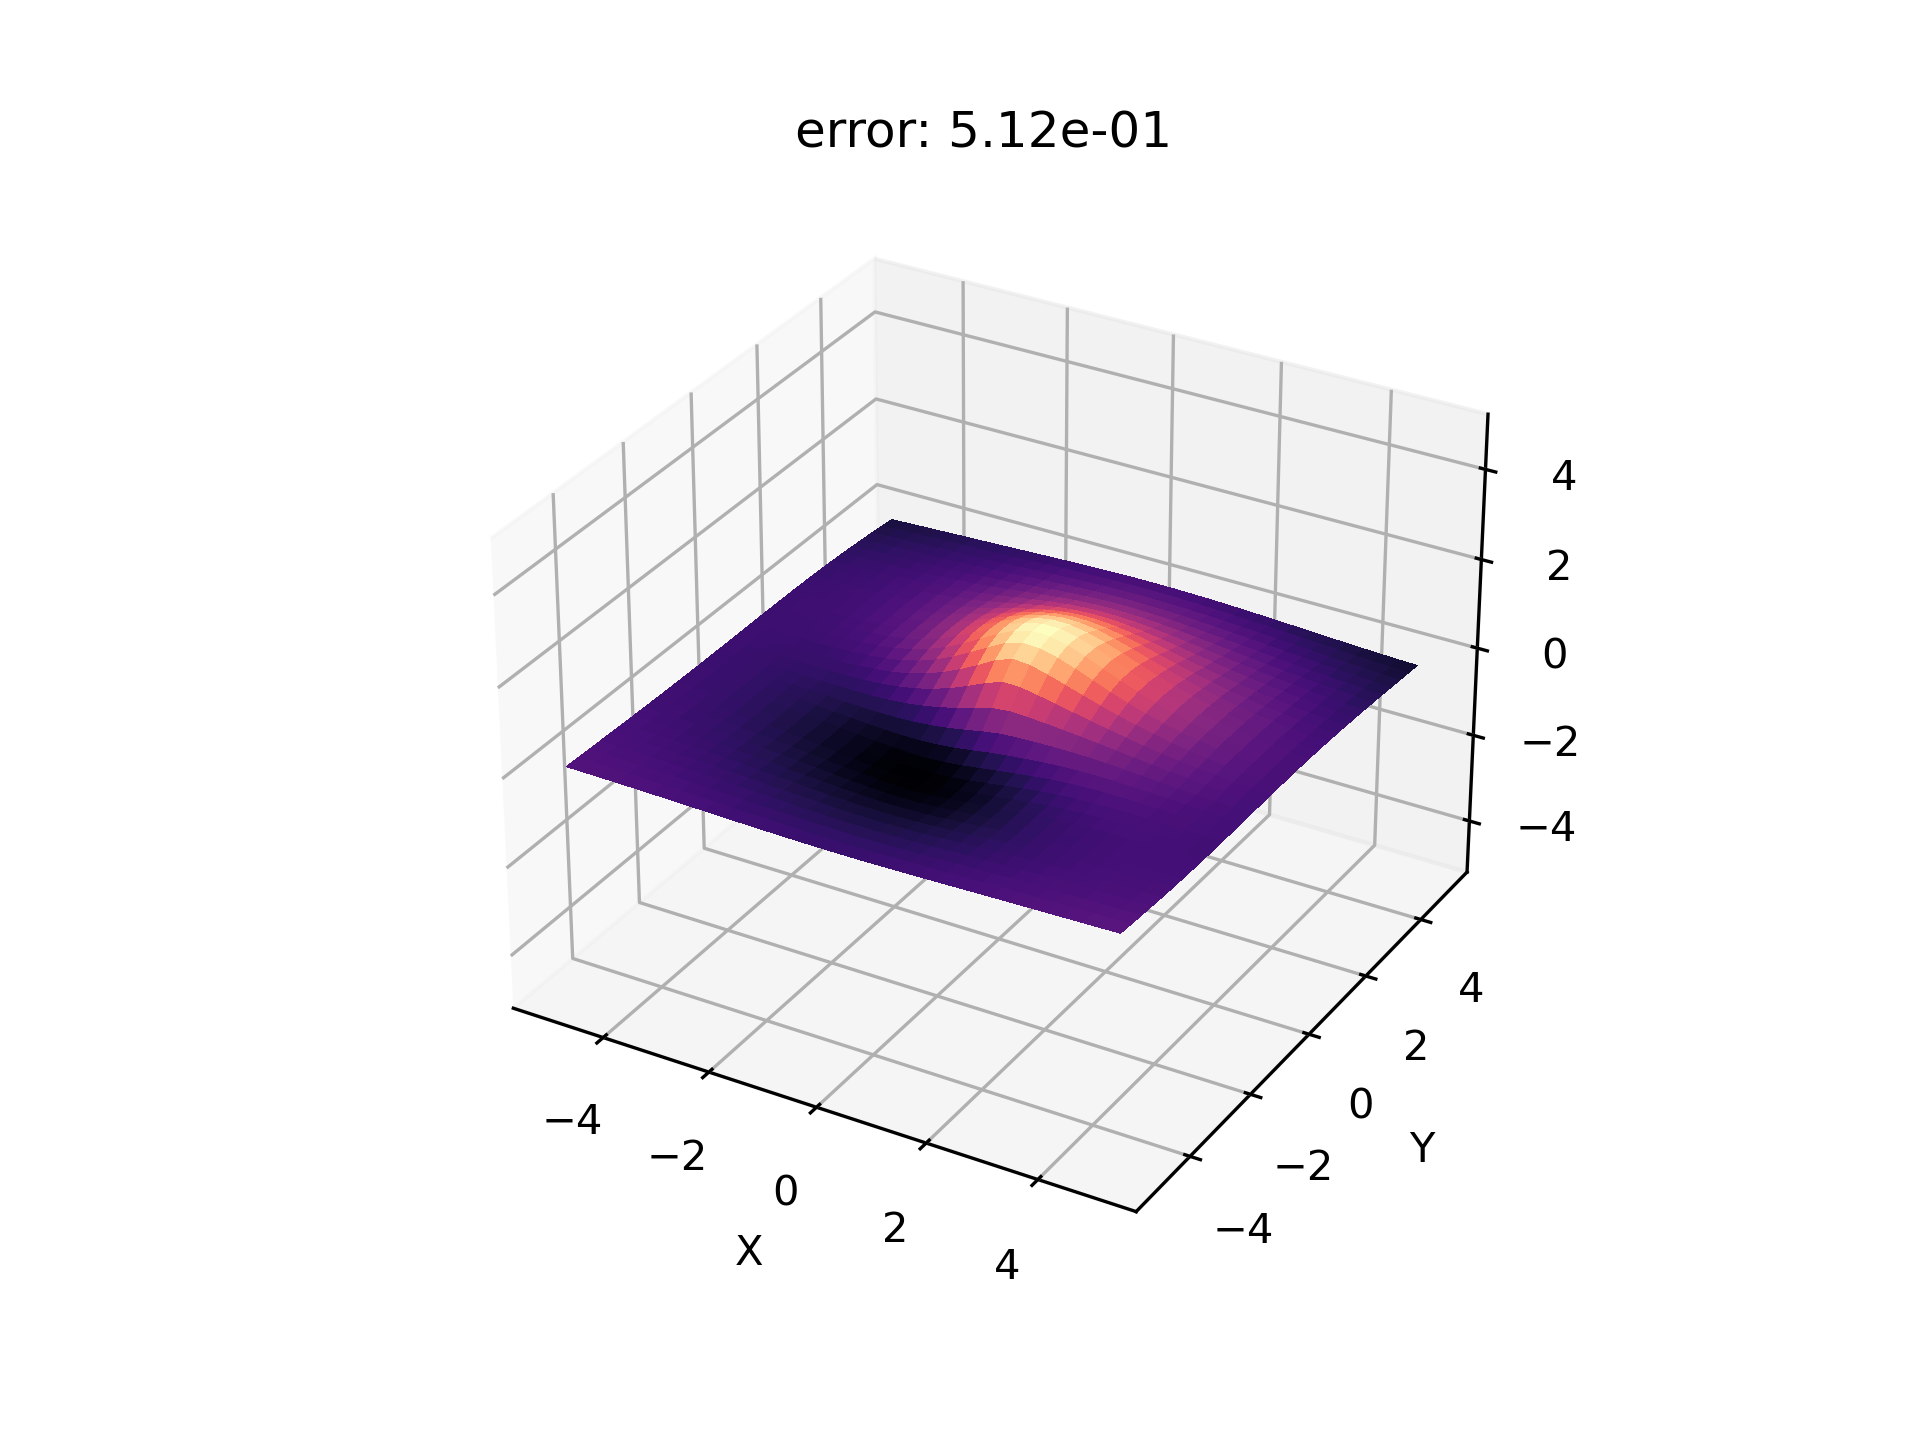
\includegraphics[width=0.3\textwidth]{Images/advection/exp1_I_32_dt_0.005_fin.png}
  \caption{Solution to the advection problem with $N=32$, $dt = 0.05$.\label{fig:adv_exp1_solution1}}
\end{figure}
\begin{figure}[H]
  \centering
  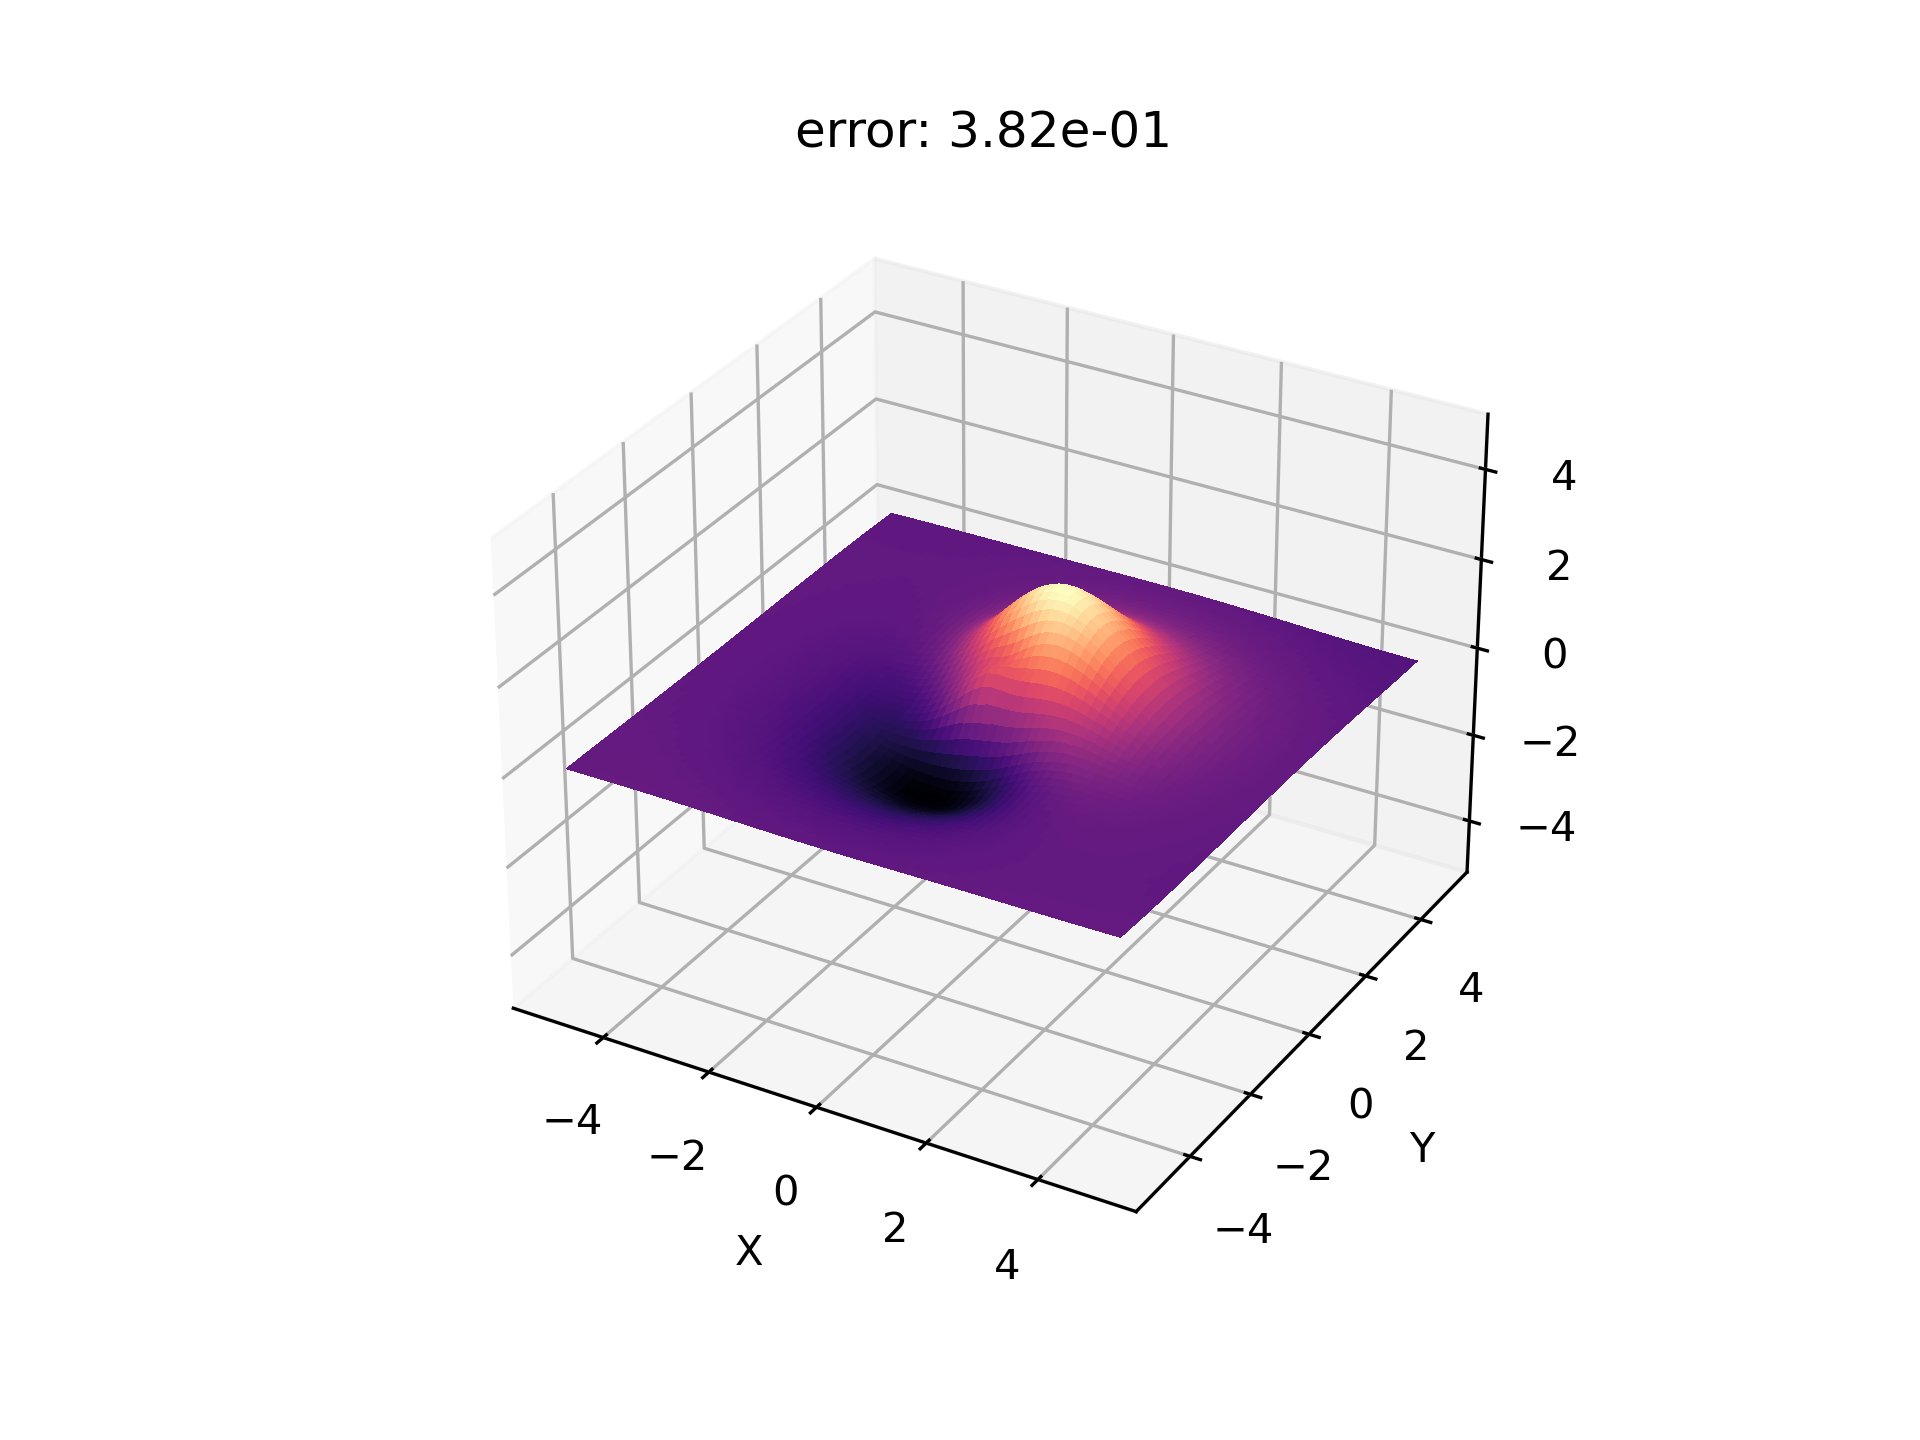
\includegraphics[width=0.3\textwidth]{Images/advection/exp1_I_64_dt_0.005_fin.png}
  \caption{Solution to the advection problem with $N=64$, $dt = 0.05$.\label{fig:adv_exp1_solution2}}
\end{figure}
\begin{figure}[H]
  \centering
  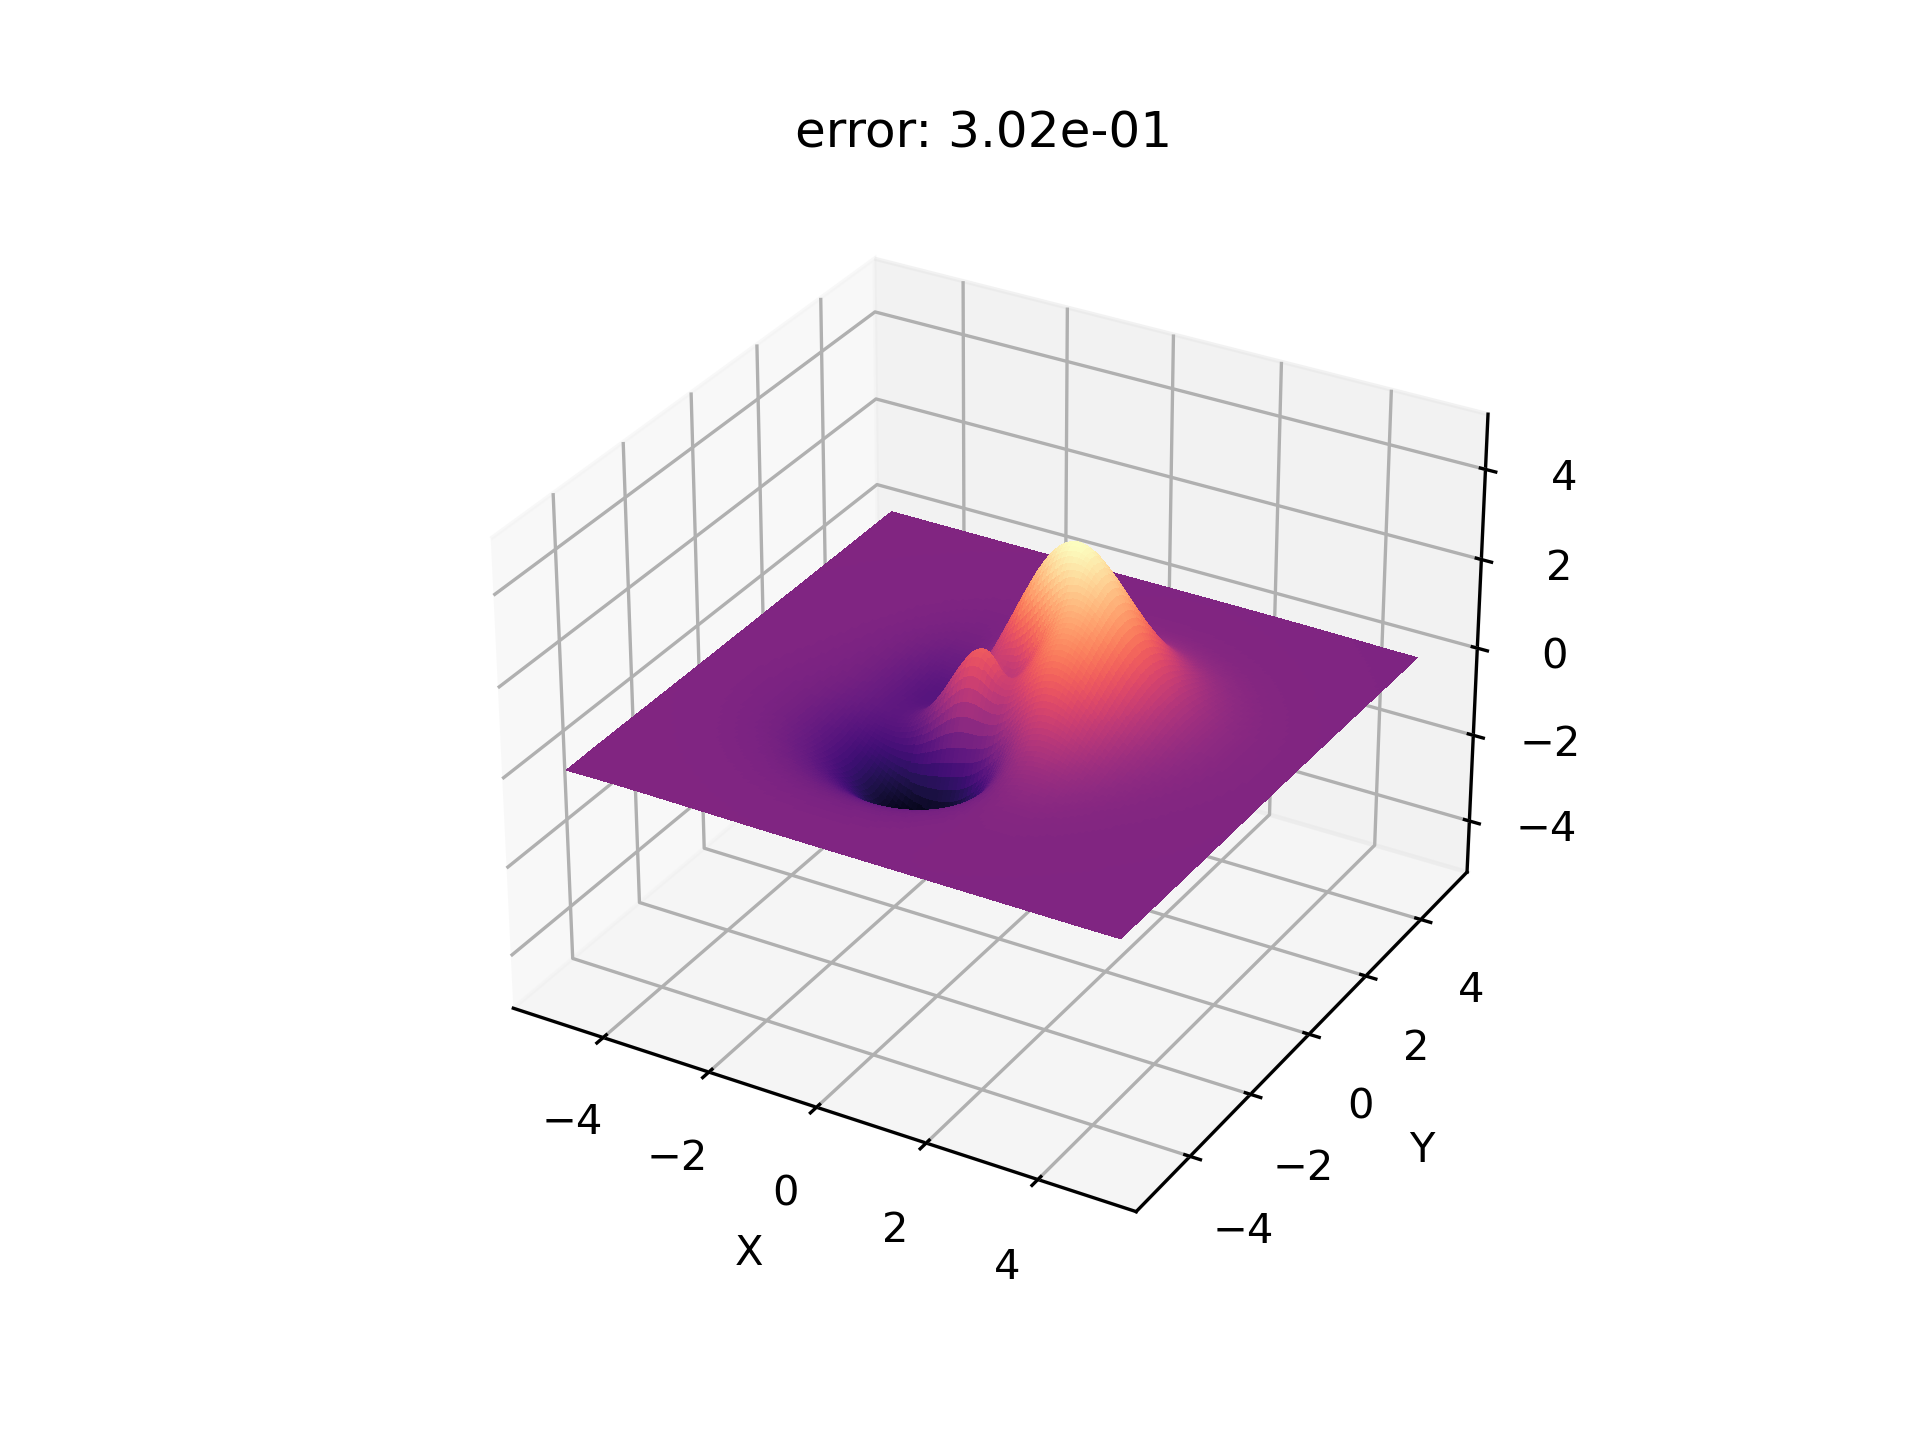
\includegraphics[width=0.3\textwidth]{Images/advection/exp1_I_128_dt_0.005_fin.png}
  \caption{Solution to the advection problem with $N=128$, $dt = 0.05$.\label{fig:adv_exp1_solution3}}
\end{figure}

It is seen from Figures~\ref{fig:adv_exp1_start}
to~\ref{fig:adv_exp1_solution3} that the peaks are eventually more pronounced
in the solutions for finer grids, just as we expected. This fits with our
expectation of errors from the mathematical model, and is therefore a
verification of our implementation.

\subsection{Experiment 2: Rotation invariance}
Another experiment we can do, is to check whether our simulation is sensitive
to symmetric inputs. Here we'll do two simulations with the same initial
conditions, but with the velocity fields rotating in opposite directions.
%
\begin{align}
  \boldsymbol u_1 & = \qty(y, -x)  \\
  \boldsymbol u_2 & = \qty(-y, x).
\end{align}
%
Ideally the error should be the same in both cases, but in reality we expect a
slight numerical error between them. Again we simulate a full rotation of the
field.

\begin{figure}[H]
  \centering
  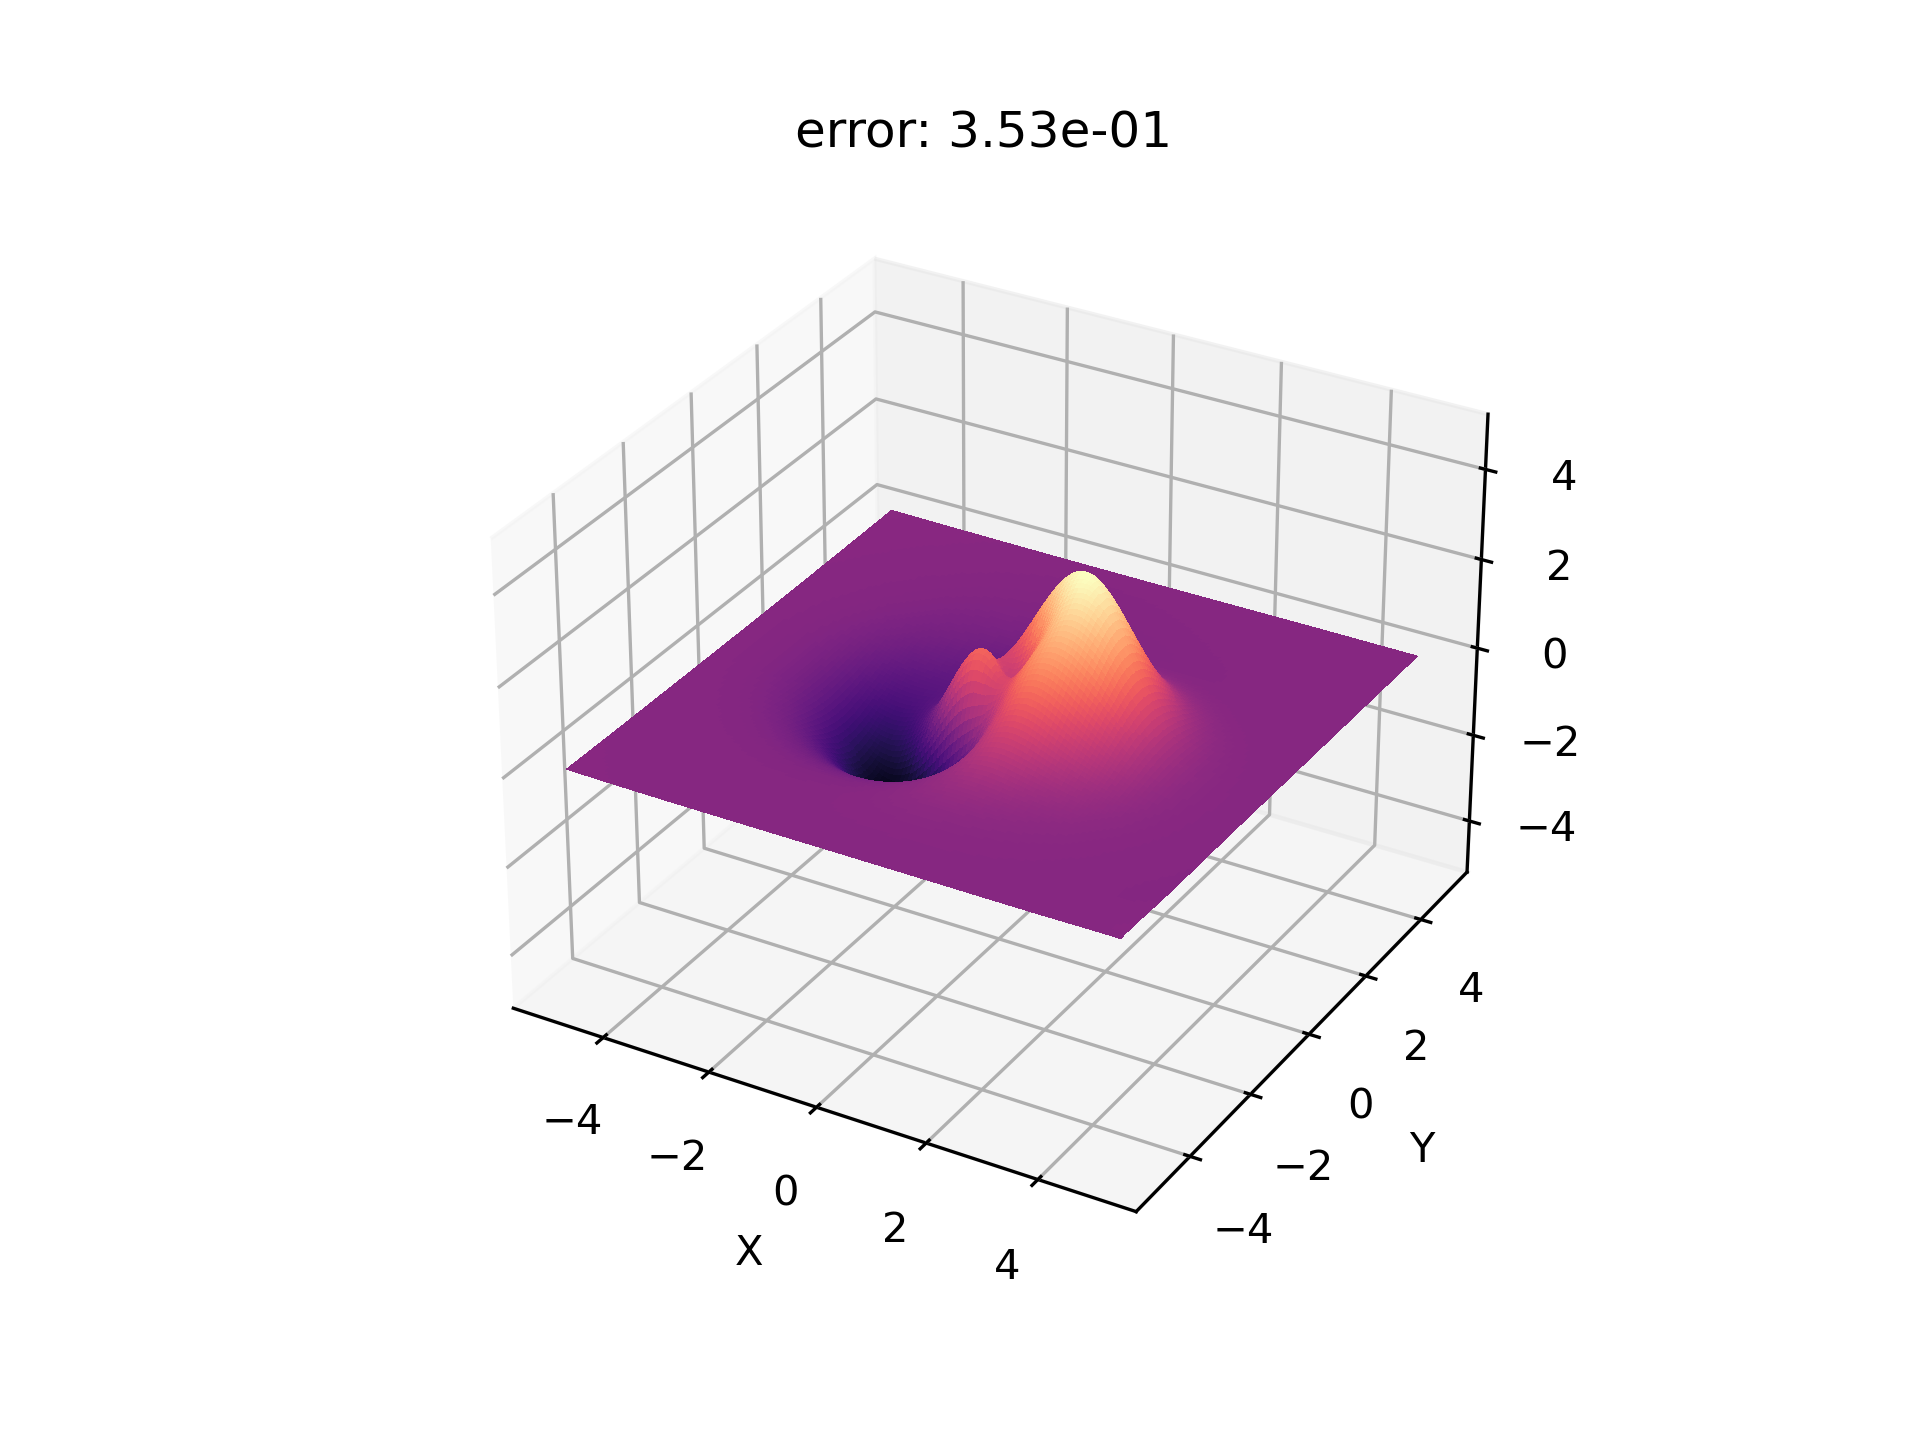
\includegraphics[width=0.3\textwidth]{Images/advection/exp2_u1.png}
  \caption{Simulation of the advection problem with the velocity field $\boldsymbol u_1 = \qty(y, -x)$.\label{fig:adv_exp2_u1}}
\end{figure}
\begin{figure}[H]
  \centering
  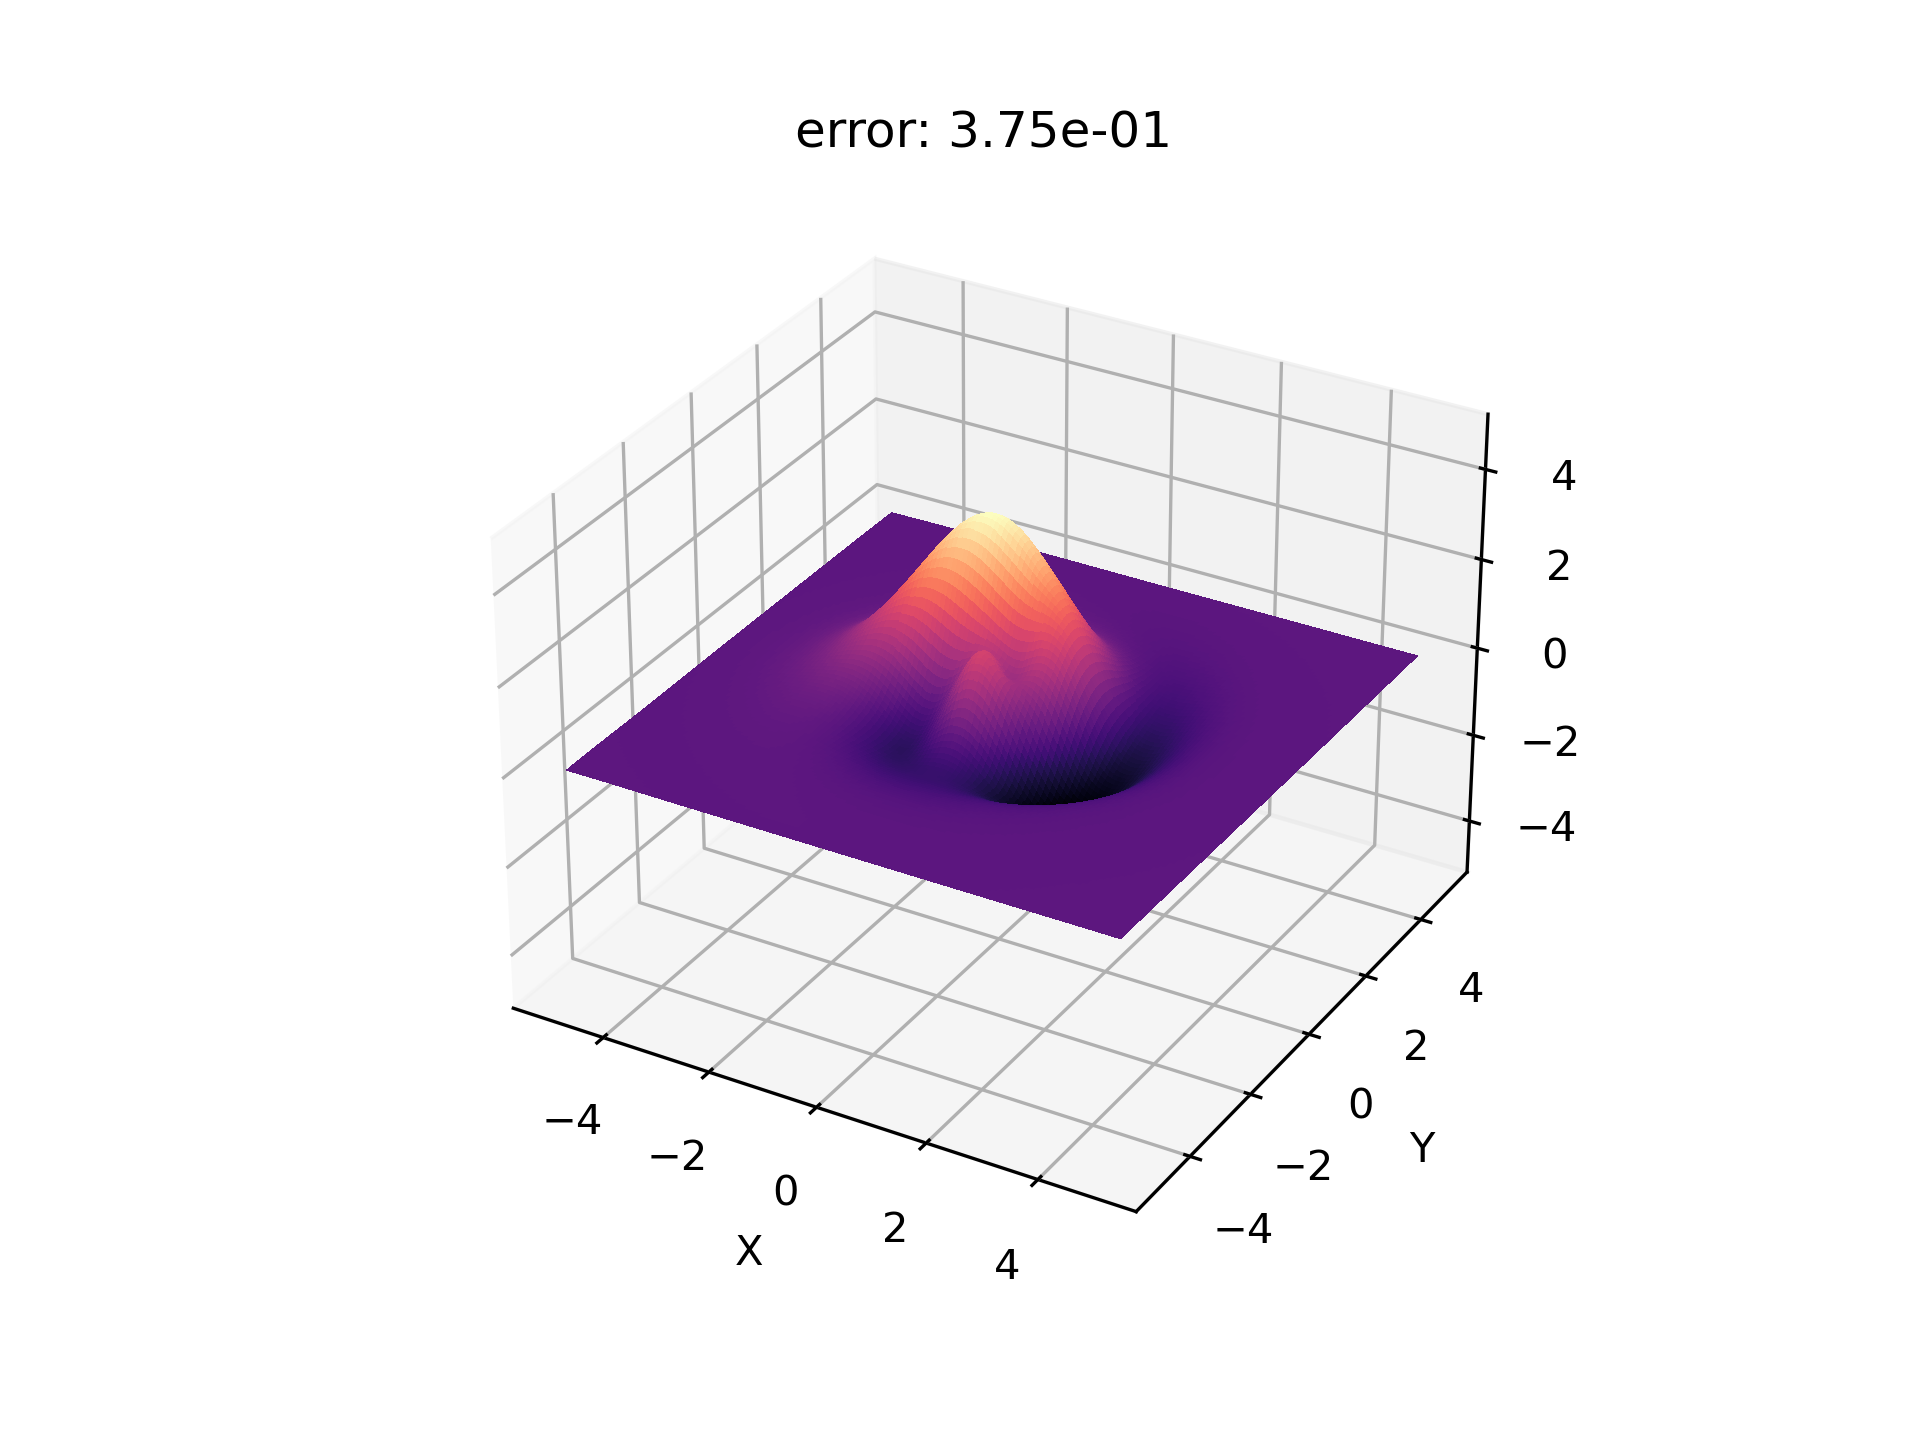
\includegraphics[width=0.3\textwidth]{Images/advection/exp2_u2.png}
  \caption{Simulation of the advection problem with the velocity field $\boldsymbol u_1 = \qty(y, -x)$.\label{fig:adv_exp2_u2}}
\end{figure}

It is seen from Figure~\ref{fig:adv_exp2_u1} and Figure~\ref{fig:adv_exp2_u2}
that the difference in the errors is on around 0.02. The error we got from the
$(128 \times 128)$ simulation in experiment 1 was around 0.4, which is much
larger. This is an ok indication that our simulation is indeed rotation
invariant. Although we'd need to do more experiments to be sure, with higher
grid values to be completely sure.

\section{Mean curvature flow}
To solve Equation (\ref{eq:mean_curvature}), we will have to rewrite $\kappa$
since we cannot directly capture the concept of a divergence operator acting on
the gradient of a field in terms of code. We refer to the slides for the
derivation. The expression for $\kappa$ is
%
\begin{align}
  \kappa = \frac{\boldsymbol \nabla \phi^T \boldsymbol \nabla \phi \, \tr(\boldsymbol H) - \boldsymbol \nabla \phi^T \boldsymbol H \boldsymbol \nabla \phi}{\left\lVert \boldsymbol \nabla \phi \right\rVert^3 },
\end{align}
%
where
%
\begin{align}
  \boldsymbol H = \begin{pmatrix}
                    \pdv[2]{\phi}{x} & \pdv{\phi}{x}{y} \\
                    \pdv{\phi}{y}{x} & \pdv[2]{\phi}{y}
                  \end{pmatrix},
\end{align}
%
is the Hessian matrix of $\phi$. We can now use the 1st and 2nd order FDA to
approximate
%
\begin{align}
  \kappa_{ij} \approx \frac{(D_x\phi_{ij})^2 D_{yy}\phi_{ij} + (D_y\phi_{ij})^2 D_{xx}\phi_{ij} - 2 D_{xy}\phi_{ij} D_x\phi_{ij} D_y\phi_{ij}}{g_{ij}^3} \label{eq:mean_curvature_FDA}
\end{align}
%
whith
%
\begin{align}
  g_{ij} = \sqrt{ (D_x \phi_{ij})^2 + (D_y \phi_{ij})^2 },
\end{align}
%
\begin{align}
  D_x \phi_{ij} & =  \frac{\phi_{i+1, j} - \phi_{i-1, j}}{\Delta x}, & D_{xx} \phi_{ij} & = \frac{\phi_{i+1, j} - 2 \phi_{ij} + \phi_{i-1, j}}{\Delta x^2}, \\
  D_y \phi_{ij} & =  \frac{\phi_{i, j+1} - \phi_{i, j-1}}{\Delta y}, & D_{yy} \phi_{ij} & = \frac{\phi_{i, j+1} - 2 \phi_{ij} + \phi_{i, j-1}}{\Delta y^2},
\end{align}
\begin{align} \quad D_{xy} \phi_{ij} & = \frac{\phi_{i+1, j+1} - \phi_{i+1, j-1} - \phi_{i-1, j+1} + \phi_{i-1, j-1}}{4 \Delta x \Delta y}.
\end{align}
%
With $\kappa$ in place, our mean curvature flow
equation~\ref{eq:mean_curvature} can be integrated using a regular explicit
Euler scheme
%
\begin{align}
  \phi_{ij}^{t+\Delta t} = \phi_{ij}^t - 2 \kappa_{ij} \Delta t. \label{eq:mean_curvature_euler}
\end{align}
%
Note that we here keep the factor 2 which is absorbed into $\Delta t$ in the
slides.

\subsection{Numerical considerations}
Looking at Equation (\ref{eq:mean_curvature_FDA}), we see that $\kappa$ might
become very large when $g_{ij} \to 0$, which in the limit might cause our
simulation to crash. To remedy this, we can fix $g_{ij}$ as to not go below a
certain value. An example could be
%
\begin{align}
  g_{ij} = \begin{cases}
             g_{ij} & \text{if } g_{ij} > 1 \\
             1      & \text{otherwise}
           \end{cases}. \label{eq:g_clamp}
\end{align}
%
Another thing we could do is to always add a small value $\epsilon$, i.e.
%
\begin{align}
  g_{ij} \to g_{ij} + \epsilon, \quad \epsilon > 0.
\end{align}
%
It is clear that, in this second case, $\epsilon$ should be chosen to be small
enough to not affect the solution, but large enough to avoid numerical
instability. We will examine the effect of these two methods in the
experiments.

Another thing we realize is that if $\phi$ is a signed distance function, the
value of $g_{ij}$ would be 1 everywhere. This is because a signed distance
function is a scalar field that assigns every point in space the distance to
the nearest point on a given surface, and is negative when inside the surface,
and since the distance to an object grows linearly in space, the spatial
derivatives are 1 everywhere.

Therefore we elect to have the initial condition for $\phi$ be a signed
distance function. There are some complications, though, in that, after just a
single integration step, we cannot be sure whether $\phi$ is still a signed
distance function, but we will ignore this for now.

Finally we need to make sure that the function we're trying to simulate doesn't
have a curvature which is too large, as then our grid might not be able to
accurately represent the geometry of the situation. The maximum curvature that
our grid can represent is $\kappa_\mathrm{max} = 1 / \max(\Delta x, \Delta y)$,
and thus we clamp the value of the curvature as such $-\kappa_\mathrm{max} \leq
  \kappa \leq \kappa_\mathrm{max}$. This can also be a problem temporally, since
the integration scheme we're using~(\ref{eq:mean_curvature_euler}) might make
$\phi$ change with a greater magnitude than the size of the grid. The maximum
curvature that our grid can represent is, as stated above, $\kappa_\mathrm{max}
  = 1 / \max(\Delta x, \Delta y)$, and thus we want
%
\begin{align}
  \kappa_\mathrm{max} < C \frac{h}{2 \Delta t},
\end{align}
%
where $h = \min(\Delta x, \Delta y)$ and $0 < C < 1$ is a constant that we can
set to control the stability of the simulation. This is called the
Courant—Friedrichs—Lewy condition. Note that the factor 2
from~(\ref{eq:mean_curvature_euler}) pops up here as well since this condition
comes directly from that equation.

\section{Experiments}
\subsection{Experiment 1: Varying $\epsilon$}
Here we examine the effect of varying the value of $\epsilon$ in the
simulation. If we set $\epsilon = 0$, we use the clamping
case~\ref{eq:g_clamp}. For initial conditions we use the signed distance
function provided in the exercise.

\begin{figure}[H]
  \centering
  \includegraphics[width=0.45\textwidth]{Images/mean_curvature/exp1_T_0.10_C_0.50_ε_0.png}
  \caption{Solution to the mean curvature problem with $T = 0.1$, $C = 0.5$, $I = 64$ and clamping $g_{ij}$.\label{fig:exp1_eps_0}}
\end{figure}
\begin{figure}[H]
  \centering
  \includegraphics[width=0.45\textwidth]{Images/mean_curvature/exp1_T_0.10_C_0.50_ε_0.01.png}
  \caption{Solution to the mean curvature problem with $T = 0.1$, $C = 0.5$, $I = 64$ and $\epsilon = 0.01$.\label{fig:exp1_eps_0.01}}
\end{figure}
\begin{figure}[H]
  \centering
  \includegraphics[width=0.45\textwidth]{Images/mean_curvature/exp1_T_0.10_C_0.50_ε_0.1.png}
  \caption{Solution to the mean curvature problem with $T = 0.1$, $C = 0.5$, $I = 64$ and $\epsilon = 0.1$.\label{fig:exp1_eps_0.1}}
\end{figure}

We see in Figure~\ref{fig:exp1_eps_0} that, in the case where we use the
clamping condition on $g_{ij}$ the discontinuities in the curvature, caused by
the discontinuities in $g_{ij}$ show up as sudden jumps in color.

In Figure~\ref{fig:exp1_eps_0.01}, where $\epsilon = 0.01$, we see that the
integration has become unstable, and as a result exhibits a checkered pattern
in the middle with extreme discontinuities in the mean curvature. This happens
since an $\epsilon$ with this value is not large enough to mitigate the
consequences of $g_{ij}$ being very small, and thus $1/(g_{ij} + \epsilon)$
blows up.

In Figure~\ref{fig:exp1_eps_0.1}, where $\epsilon = 0.1$, we see that this
problem has been solved. The mean curvature field is now smooth and continuous,
meaning that we've hit a sweet spot with $\epsilon$. It should be said that
even though the clamping case exhibits discontinuities, it's only inside the
object, and thus the solution outside should be just as valid as the one for
$\epsilon = 0.1$, which is also apparent in the contour plots in the two
figures for these cases, which are very similar.

\subsection{Experiment 2: Varying the grid size}
As with all numerical simulation and as also touched upon numerous times in
this report, the grid fineness is a crucial parameter to achieving accuracy.
Here we will examine the effect of varying the grid size on the solution of the
mean curvature problem. We again use the initial conditions provided in the
exercise.

\begin{figure}[H]
  \centering
  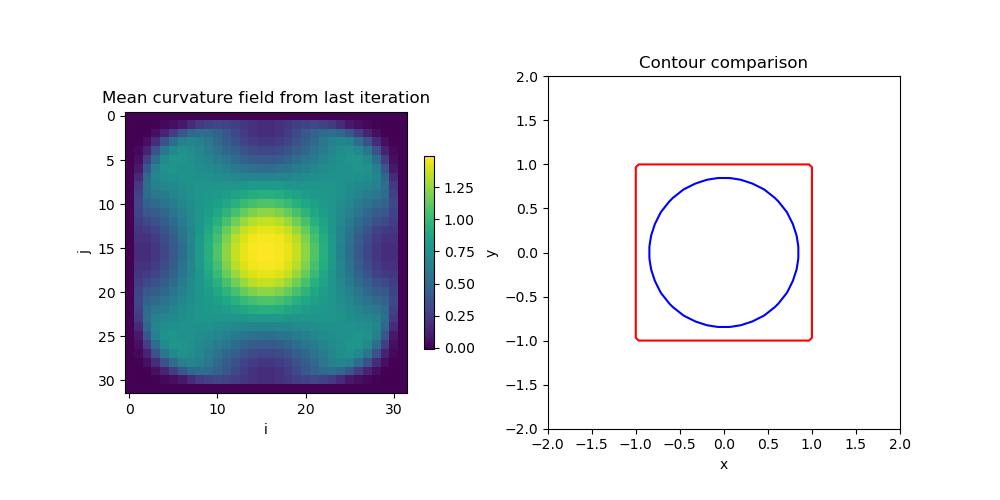
\includegraphics[width=0.45\textwidth]{Images/mean_curvature/exp2_I_32.png}
  \caption{Solution to the mean curvature problem with $T = 0.1$, $C = 0.25$, $\epsilon = 0.05$ and $I = 32$.\label{fig:exp2_I_32}}
\end{figure}
\begin{figure}[H]
  \centering
  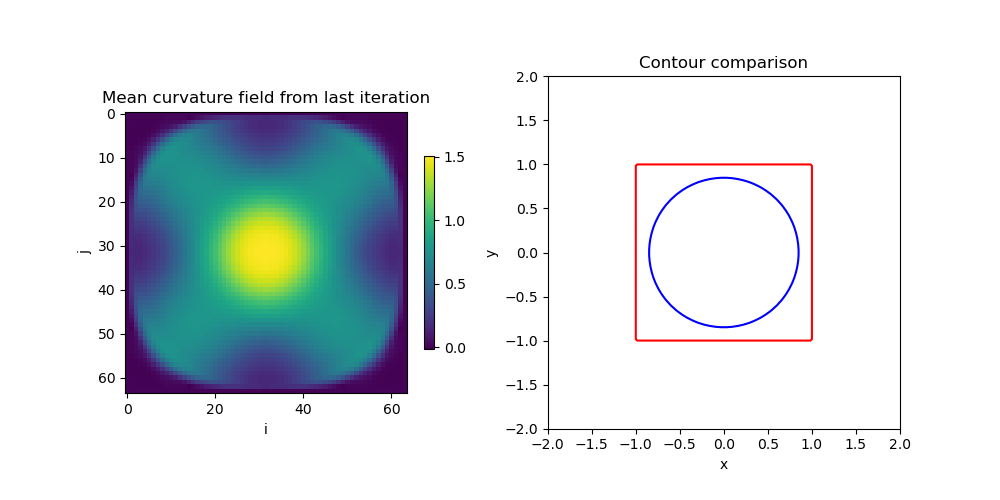
\includegraphics[width=0.45\textwidth]{Images/mean_curvature/exp2_I_64.png}
  \caption{Solution to the mean curvature problem with $T = 0.1$, $C = 0.25$, $\epsilon = 0.05$ and $I = 64$.\label{fig:exp2_I_64}}
\end{figure}
\begin{figure}[H]
  \centering
  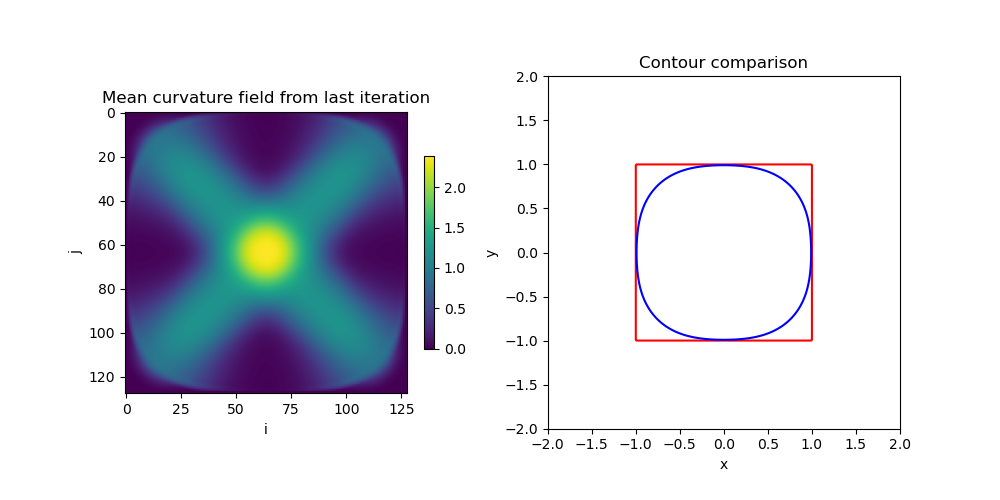
\includegraphics[width=0.45\textwidth]{Images/mean_curvature/exp2_I_128.png}
  \caption{Solution to the mean curvature problem with $T = 0.1$, $C = 0.25$, $\epsilon = 0.05$ and $I = 128$\label{fig:exp2_I_128}}
\end{figure}

We see in Figures~\ref{fig:exp2_I_32} to~\ref{fig:exp2_I_128} that already
after $T=0.1$, the solution is indeed sensitive to the grid fineness. This is
especially seen in the respective contour plots. Here, the finest grid with
$N=128$ is still retaining some of the original square shape, while the other
two cases have already colapsed into spheres. The coarsest grid with $N = 32$
even even has slight bumps on the circle showcasing it's inferior precision.

These observation fit with our mathematical predictions of the errors, and is
therefore a verification of our implementation.

\subsection{Experiment 3: A rectangle}
In this experiment we will examine the effect the assymmetry of an object on
the local mean curvature and thus the speed of shrinking due to the
integration. For initial conditions replace the square with a rectangle with
sides $3$ and $1/3$. We will use the values $I = 64$, $T = 0.1$, $C = 0.1$, and
$\epsilon = 0.1$, and plot the same solution in three steps of length $t = T/3$
each. We expect the short side to shrink faster than the long side because the
curvature will be greatest here.

\begin{figure}
  \centering
  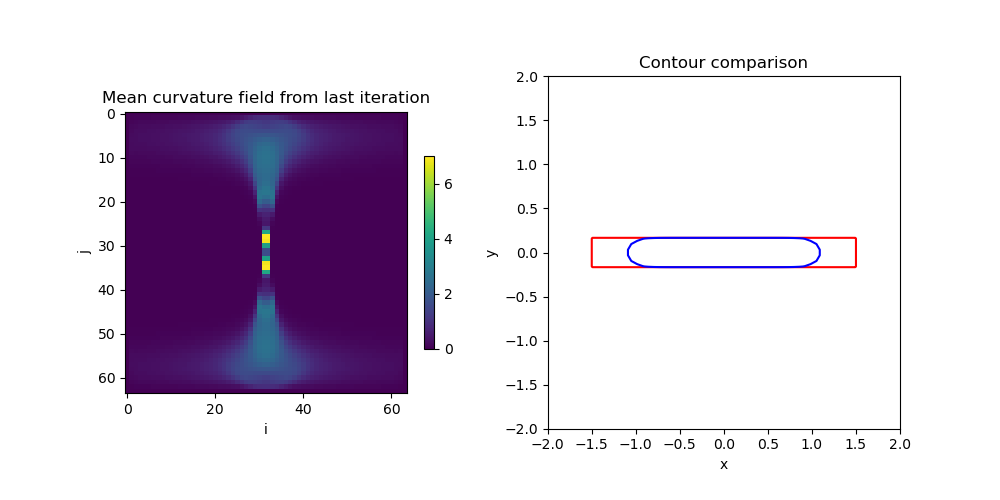
\includegraphics[width=0.45\textwidth]{Images/mean_curvature/exp3_step_1.png}
  \caption{First step of the solution to the mean curvature problem with a rectangular polygon.\label{fig:exp3_step_1}}
\end{figure}
\begin{figure}
  \centering
  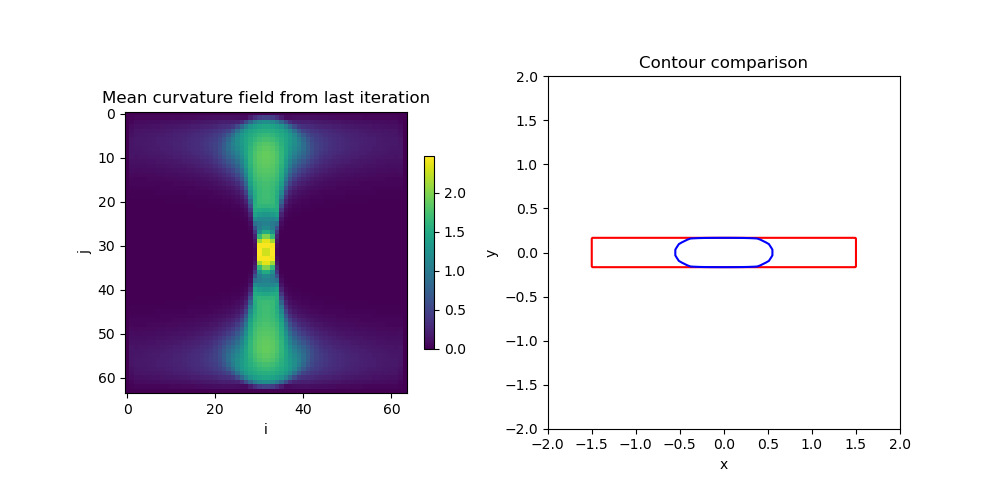
\includegraphics[width=0.45\textwidth]{Images/mean_curvature/exp3_step_2.png}
  \caption{Second step of the solution to the mean curvature problem with a rectangular polygon.\label{fig:exp3_step_2}}
\end{figure}
\begin{figure}
  \centering
  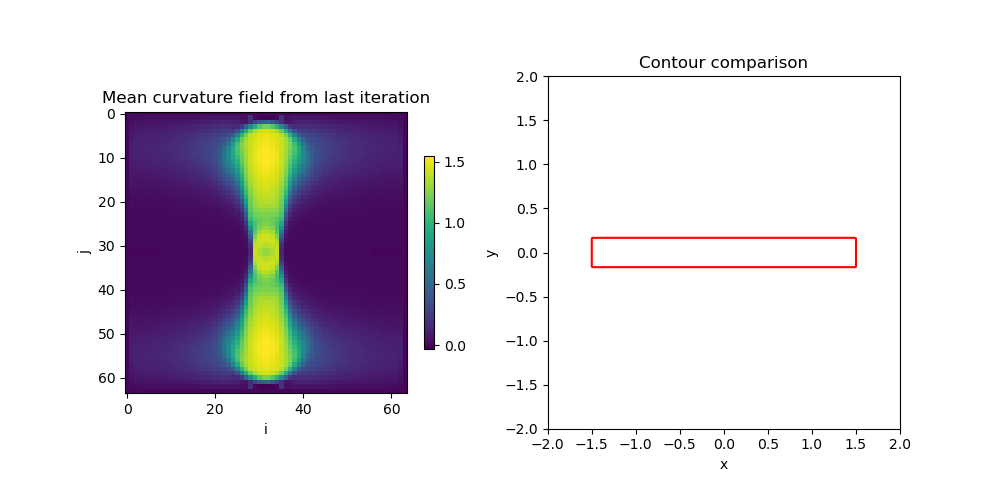
\includegraphics[width=0.45\textwidth]{Images/mean_curvature/exp3_step_3.png}
  \caption{Third step of the solution to the mean curvature problem with a rectangular polygon.\label{fig:exp3_step_3}}
\end{figure}

We see that the curvature is larger on the short side, and thus the short side
shrinks faster than the long side, just as expected. This fits with the
mathematical model, and is therefore a verification of our implementation.

\end{document}
\endinput
